%!TEX root = ../main.tex
\label{sec:ILDTiming}

The timing of hits is registered in a very simplified way as explained in section \ref{subsec:ILDDigiCalo}. Different time windows ranging from 1 ns to 100 ns are used. This is done to evaluate the effects of such timing window on the reconstruction of hadronic showers. To generate hadronic showers almost exclusively inside the hadronic calorimeter, neutral kaons particles (\kzeroL{}) are used with energies ranging from 5 GeV to 90 GeV, corresponding typically to the energy range of particles inside a jet of energies between 50 to 250 GeV. The kaons are projected exclusively inside the barrel at a direction (0.5, 0.5, 0.1) corresponding to the middle of an ILD HCAL stave at angles $\theta$ between 0 and 35 degrees and $\phi$ up to 360 degrees. This is done to avoid the barrel-endcap transition and keep the generic nature of the results. The QGSP\_BERT\_HP physics list is used to simulate hadronic showers.

\section{Check of the energy reconstruction}

Before studying the effect of timing on hadrons showers, it is important to check the energy reconstruction of the ILD detector with the initially provided calibration constants. The energy is initially reconstructed by scaling the hit energy of calorimeters with various constants. The main important ones are:
\begin{itemize}
  \item A constant used for converting the energy from GeV to MIP. For the HCAL, the constant is \textit{CalibHCALMIP} and is equal to 497.5 keV/MIP.
  \item The light yield constant used to convert MIP to pixels. For the HCAL, this constant is equal to 15 pixel per MIP.
  \item A constant used for the scaling of the reconstructed hit energy due to the sampling fraction of the calorimeters. For example, the \textit{CalibrHCALBarrel} constant is responsible for the sampling fraction in the HCAL barrel and is equal to 50.8262.
\end{itemize}

In a next step, the digitized hits are passed on to PandoraPFA. Several energy reconstruction schemes can be done with PandoraPFA:
\begin{itemize}
  \item Simple energy reconstruction: The energy of all hits belonging to a cluster are added.
  \item Energy truncation: The energy of a cell is truncated when it is over 1 GeV \cite{Tran:2017tgr}.
  \item Software compensation (SC): the EM and HAD component of a shower are weighted to correct for non-compensation nature of the AHCAL \cite{Tran:2017tgr}.
  \item Non-linearity correction (NLC): a correction is applied to the cluster energy to account for non-linearity effects introduced by PandoraPFA.
\end{itemize}
However, the calibration constants used by PandoraPFA need to be prior calibrated. The calibration procedure is explained in \cite{PandoraCalib}. To cross-check the energy calibration, the calorimeter linearity and energy resolution have been investigated. Both have been looked at the hit level, i.e. before PandoraPFA and at the cluster level, i.e. after PandoraPFA. The same procedure as described in \textit{Pandora Analysis} package is used to determine the energy resolution defined as RMS$_{90}$/Mean$_{90}$. RMS$_{90}$ and Mean$_{90}$ are from a gaussian fit in the smallest range of total reconstructed energy which contains 90\% of all events. This makes the energy resolution from single particles directly comparable to the energy resolution of the CALICE AHCAL \cite{Tran:2017tgr, SoftCompNew2012}, which is determined from gaussian fits to the reconstructed energy. Only events in the barrel ($|\cos\theta| < 0.7$) and with a single reconstructed Particle Flow Object (PFO) are selected for this cross-check.

Figures \ref{fig:linhits} and \ref{fig:resohits} show the linearity and resolution curves for different cases, in all cases, the reconstructed energy is obtained by summing up the energy of all calorimeter hits. The blue and black curves, representing the cases where software compensation or energy truncation are used, are similar as well as the green and red curves, representing the case where the energy truncation and the non-linearity correction are used after a recalibration of the PandoraPFA calibration constants has been performed. This is because the energy reconstruction scheme does not affect the calorimeter hit energy. The blue and black curves deviate from linearity due to mis-calibrated hit energy scaling constants. The linearity curve varies between -5\% and 5\% and also crosses the line $x=y$ which if corrected would degrade the energy resolution. The red and green curves are obtained after the recalibration of the hit energy scaling constants therefore differ from the blue and black curves. The non-linearity correction does not have an effect on the reconstructed energy because it is only applied to clusters. The linearity fluctuates between -10\% and 0\% but does not cross the line $x=y$. Looking at the energy resolution, all the curves are very similar. The recalibration of the scaling constants improves slightly the energy resolution by around 1\%. This cross-check shows that the hit energy scaling constants have a large influence ($\sim$5\%) on the energy linearity of the calorimeter. However, the effect is relatively small ($\sim$1\%) on the energy resolution of the calorimeter.

\begin{figure}[htbp!]
  \centering
  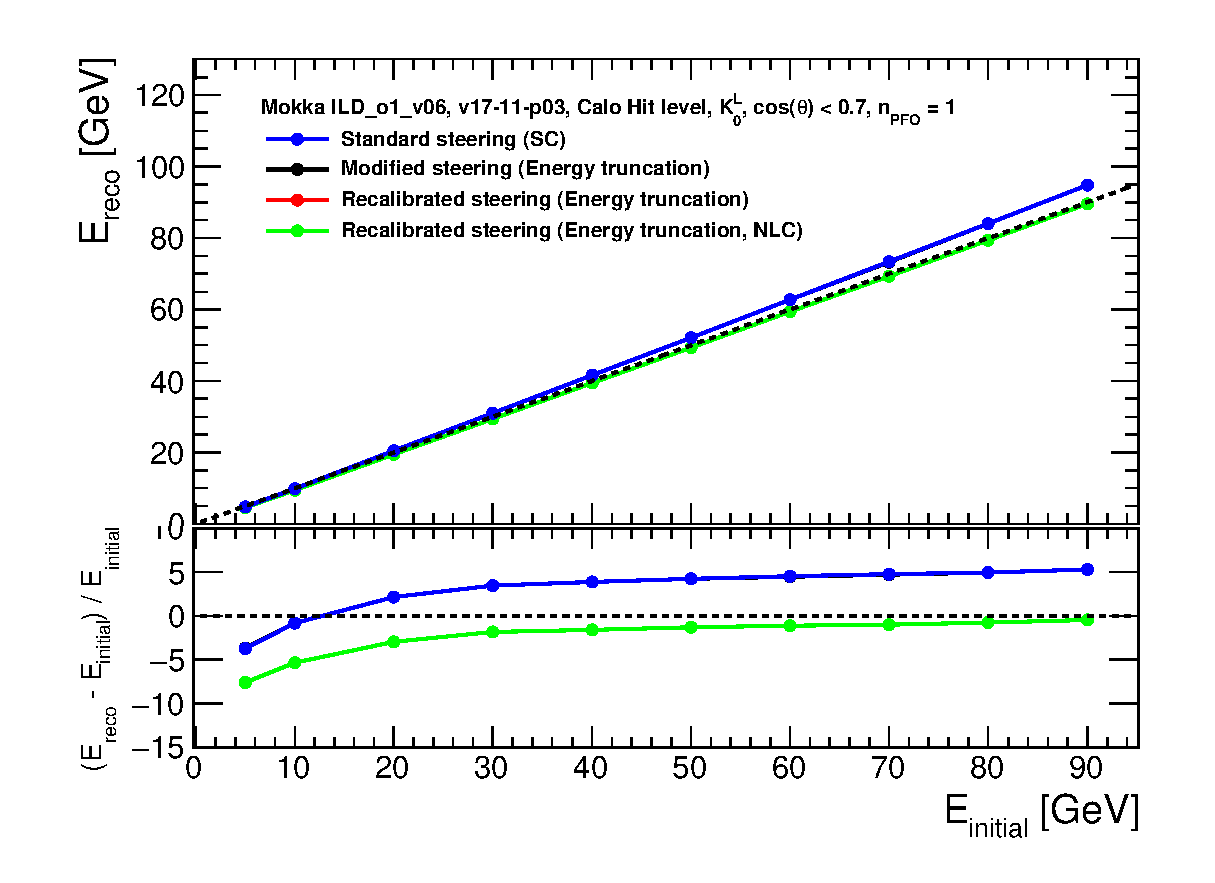
\includegraphics[width=0.6\linewidth]{../Thesis_Plots/ILD/CheckCalib/Comparison_linearity_Curves_Hits.eps}
  \caption{Mean reconstructed energy $E_{reco}$ for 5 to 90 GeV \kzeroL{} as a function of the simulated energy $E_{initial}$. The reconstructed energy is the sum of all calibrated hit energies. The bottom plot shows the relative deviation from linearity. Error bars represent the statistical uncertainty. The black and blue curves represent the cases where software compensation or energy truncation reconstruction scheme is used and are the same. The red and green curve are the same, representing the case where the energy truncation and the non-linearity correction reconstruction scheme are used after a recalibration of the PandoraPFA calibration constants has been performed.} \label{fig:linhits}
\end{figure}

\begin{figure}[htbp!]
  \centering
  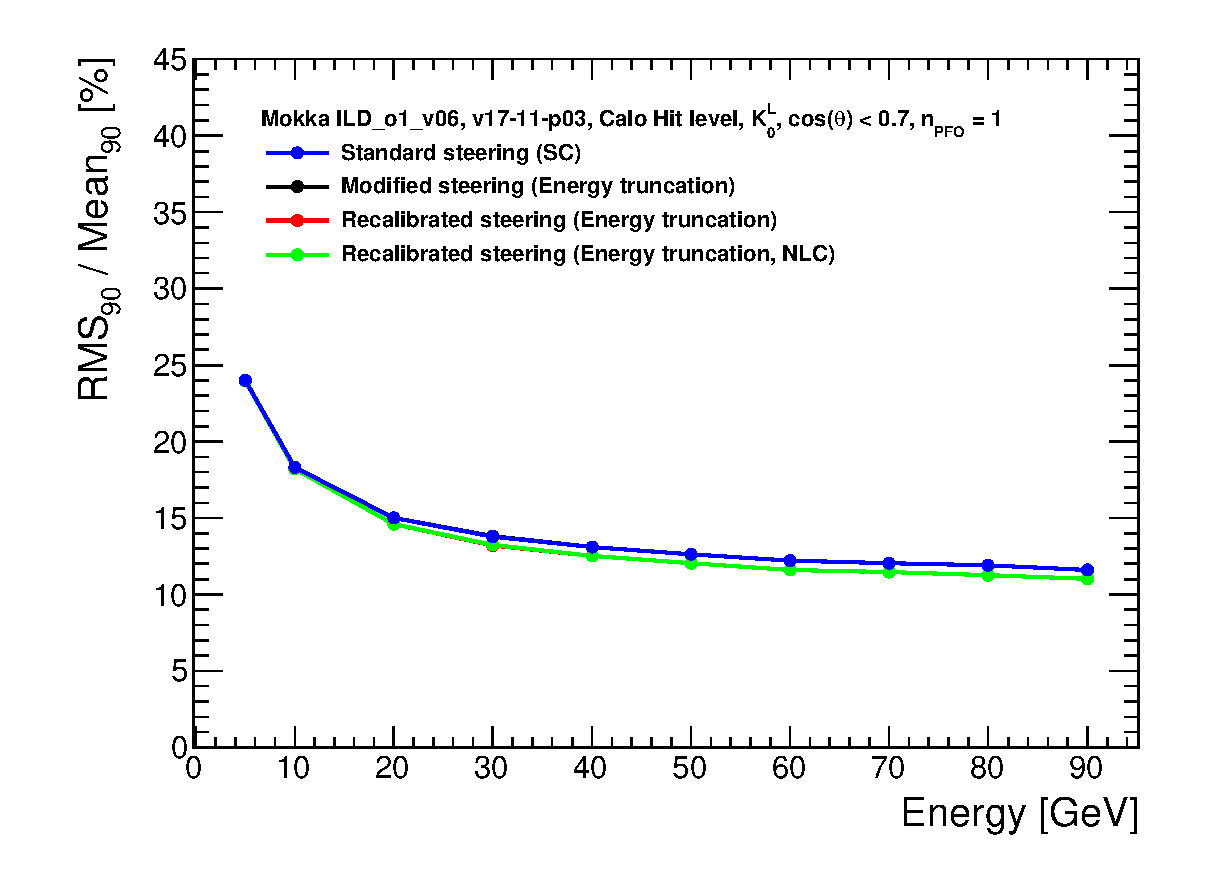
\includegraphics[width=0.6\linewidth]{../Thesis_Plots/ILD/CheckCalib/Comparison_resolution_Curves_Hits.eps}
  \caption{Relative energy resolution RMS$_{90}$/Mean$_{90}$ as a function of the energy. Error bars represent the statistical uncertainty. The black and blue curves are the same and the red and green curve are the same.} \label{fig:resohits}
\end{figure}

Figures \ref{fig:linpfo} and \ref{fig:resopfo} shows the linearity and resolution curves for different energy reconstruction schemes after PandoraPFA. By comparing these figures to the one shown above, it enables to understand the effects of the different energy reconstruction schemes in PandoraPFA. The reconstructed energy is the energy of the reconstructed PFO. For the linearity curve, the red and black lines in the case of energy truncation reconstruction scheme are similar and show a non-linearity especially at high energies between -10\% and 2\%. It shows that the energy truncation introduces a non-linearity effect on the energy reconstruction. The difference between the curves could be related to the difference of the hit energy scaling constant. However, it has a small effect around 1-2\% that may come from the clustering step in PandoraPFA. The green curve in the case of energy truncation and non-linearity correction reconstruction scheme shows a linear behavior. The blue curve in the case of software compensation reconstruction scheme deviates from the linearity by around 10\%. This is believed to be related to the software compensation weights applied in the reconstruction scheme that were not optimized for this ILD model. Regarding the resolution curves, a very small rise ($\sim$ 1-2\%) of the resolution at high energies of the black, red and green curves is visible. As expected, a degradation of the energy resolution is observed where the non-linearity correction is applied. In the software compensation reconstruction scheme, a slight change in the curve can be seen at 50 GeV. This is correlated with the change of the curve slope in the linearity plot.

Despite that the energy linearity is not perfect, the energy reconstruction, after the recalibration of the different constants used in the reconstruction, is good enough to study the impact of timing cuts on hadronic showers. In the following analysis, the different hadronic shower variables will be obtained at the individual hit level. This is done in order to avoid clustering effects from PandoraPFA.

\begin{figure}[htbp!]
  \centering
  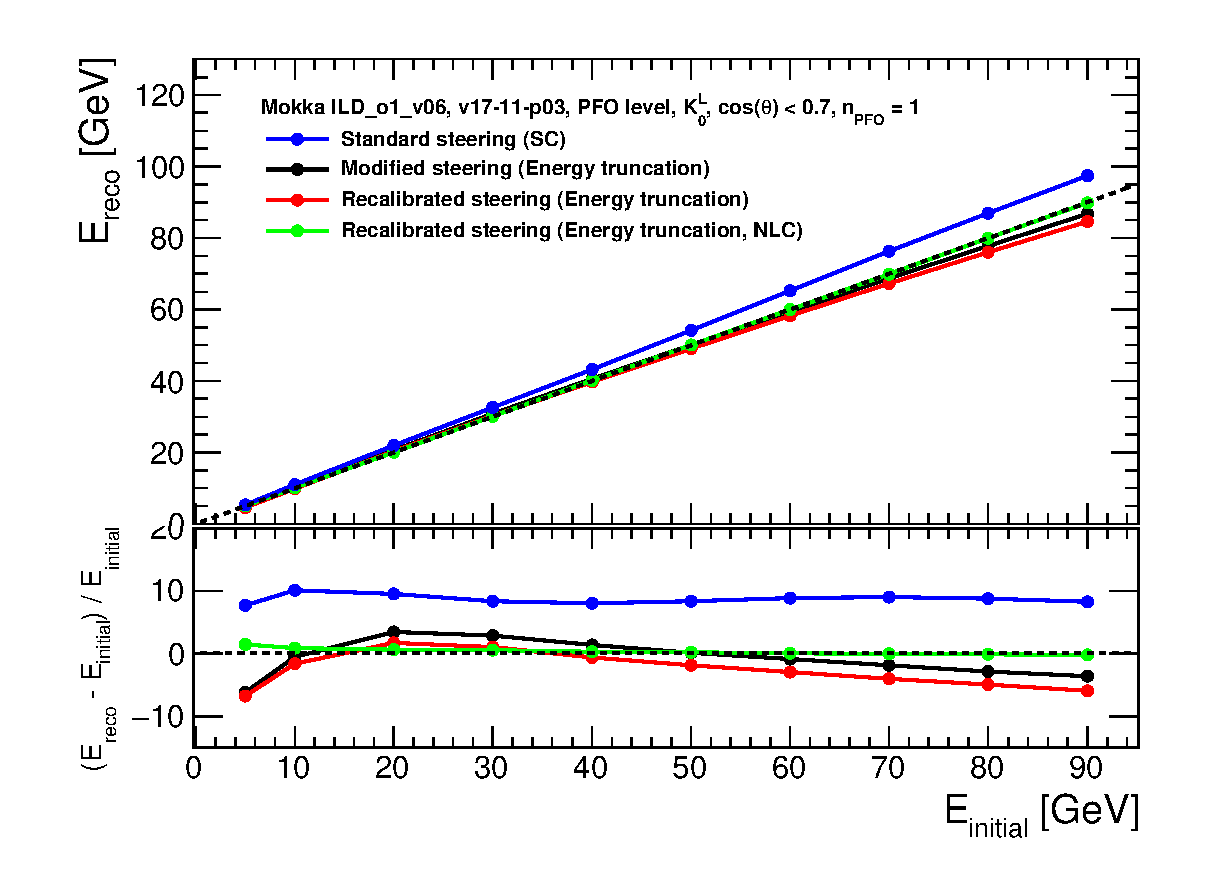
\includegraphics[width=0.6\linewidth]{../Thesis_Plots/ILD/CheckCalib/Comparison_linearity_Curves_PFO.eps}
  \caption{Mean PFO reconstructed energy $E_{reco}$ for 5 to 90 GeV \kzeroL{} as a function of the simulated energy $E_{initial}$ for different energy reconstruction schemes. The bottom plot shows the relative deviation from linearity. Error bars represent the statistical uncertainty.} \label{fig:linpfo}
\end{figure}

\begin{figure}[htbp!]
  \centering
  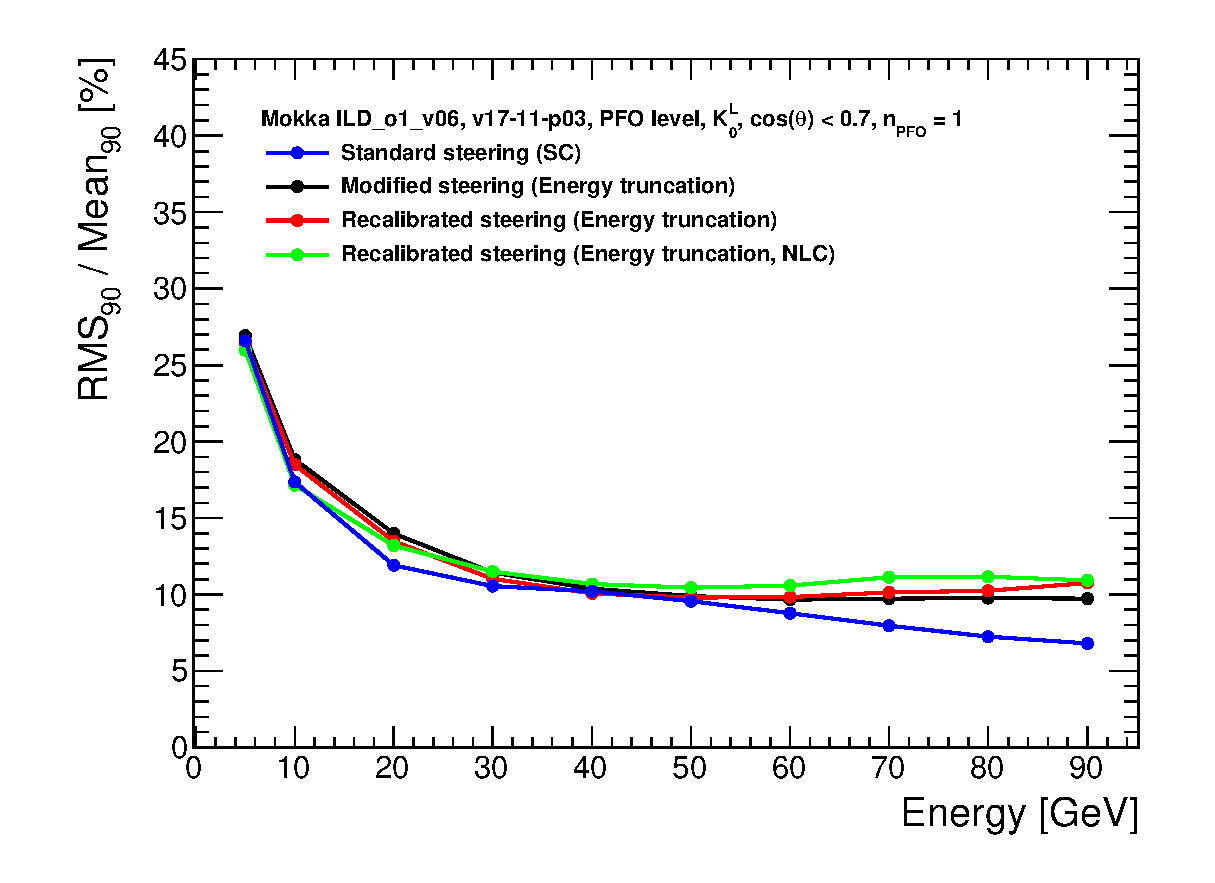
\includegraphics[width=0.6\linewidth]{../Thesis_Plots/ILD/CheckCalib/Comparison_resolution_Curves_PFO.eps}
  \caption{Relative PFO energy resolution RMS$_{90}$/Mean$_{90}$ as a function of the energy for different energy reconstruction schemes. Error bars represent the statistical uncertainty.} \label{fig:resopfo}
\end{figure}

\section{Influence of timing cuts on hadronic showers in the ILD detector}
\label{sec:MCLevelILDTiming}

\subsection{Motivation}

To illustrate typical topological situation, the figure \ref{fig:Motivation} shows the momenta distribution and distances of two classes of events: for jets representative of heavy boson decay near production threshold \ee{}\ra{} \Zqq{} with $q = u,d,s$ and for heavy boosted jets with a more complex event topology \ee{}\ra{} \WWqqqq{} where q is a quark. They show that typically the momentum spectrum is dominated by low momenta below 10-20 GeV while the minimal distance (measured at the front face of the SiW-ECAL) between a charged and neutral hadron changes greatly depending of the center of mass energy.

In the case of the production of a Z boson near threshold, the mean distance is around \SI{180}{\milli\meter} thus in this context, showers are well separated. However at higher energies where density is higher, typical distances of \SI{50}{\milli\meter} need to be resolved. This situation can become relevant in the contribution of confusion to the jet energy resolution. In this case, the use of timing information could help to separate nearby showers and improve the pattern recognition.

\begin{figure}[htbp!]
  \centering
  \begin{subfigure}[t]{0.49\textwidth}
    \centering
    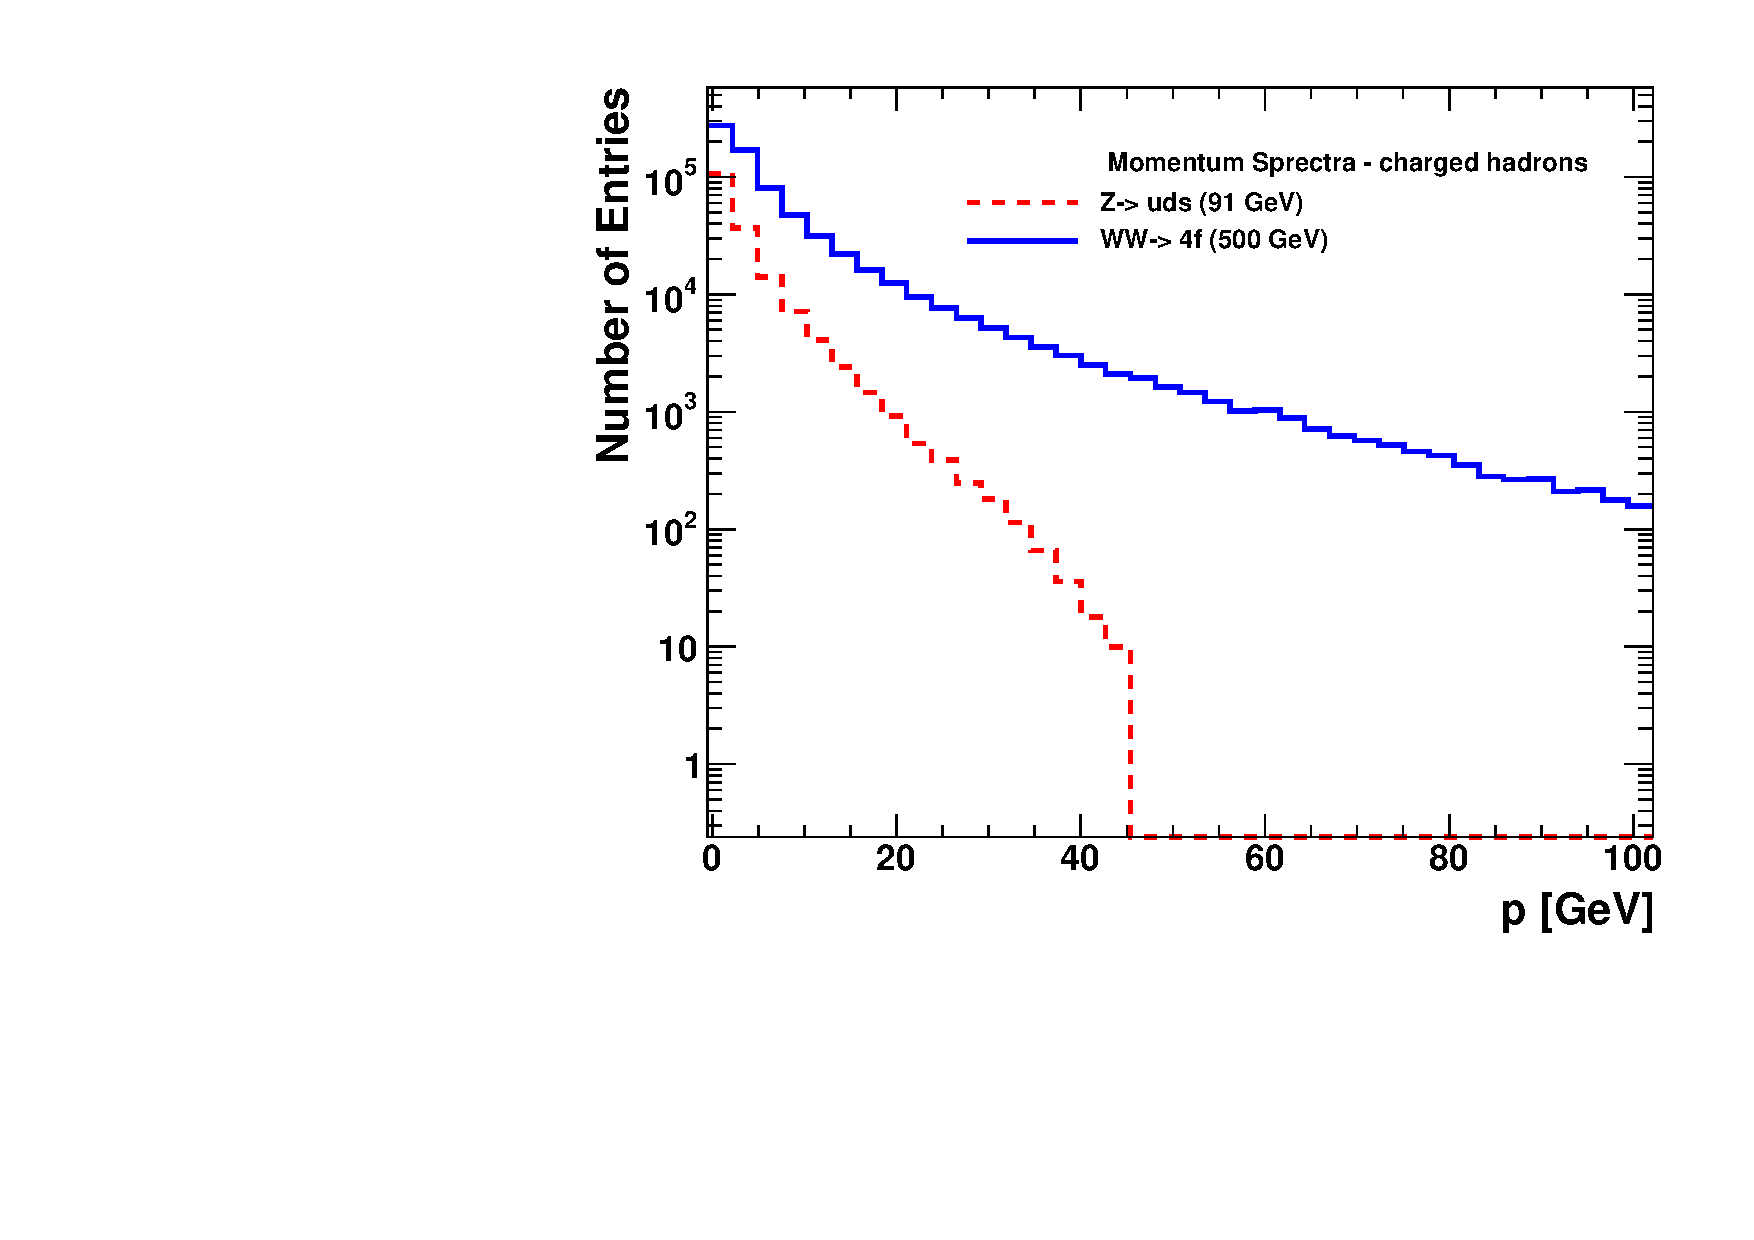
\includegraphics[width=1\linewidth]{../Thesis_Plots/ILD/Momentum_spectra_to100GeV_final.pdf}
    \caption{} \label{fig:momentumparticlejets}
  \end{subfigure}
  \hfill
  \begin{subfigure}[t]{0.49\textwidth}
    \centering
    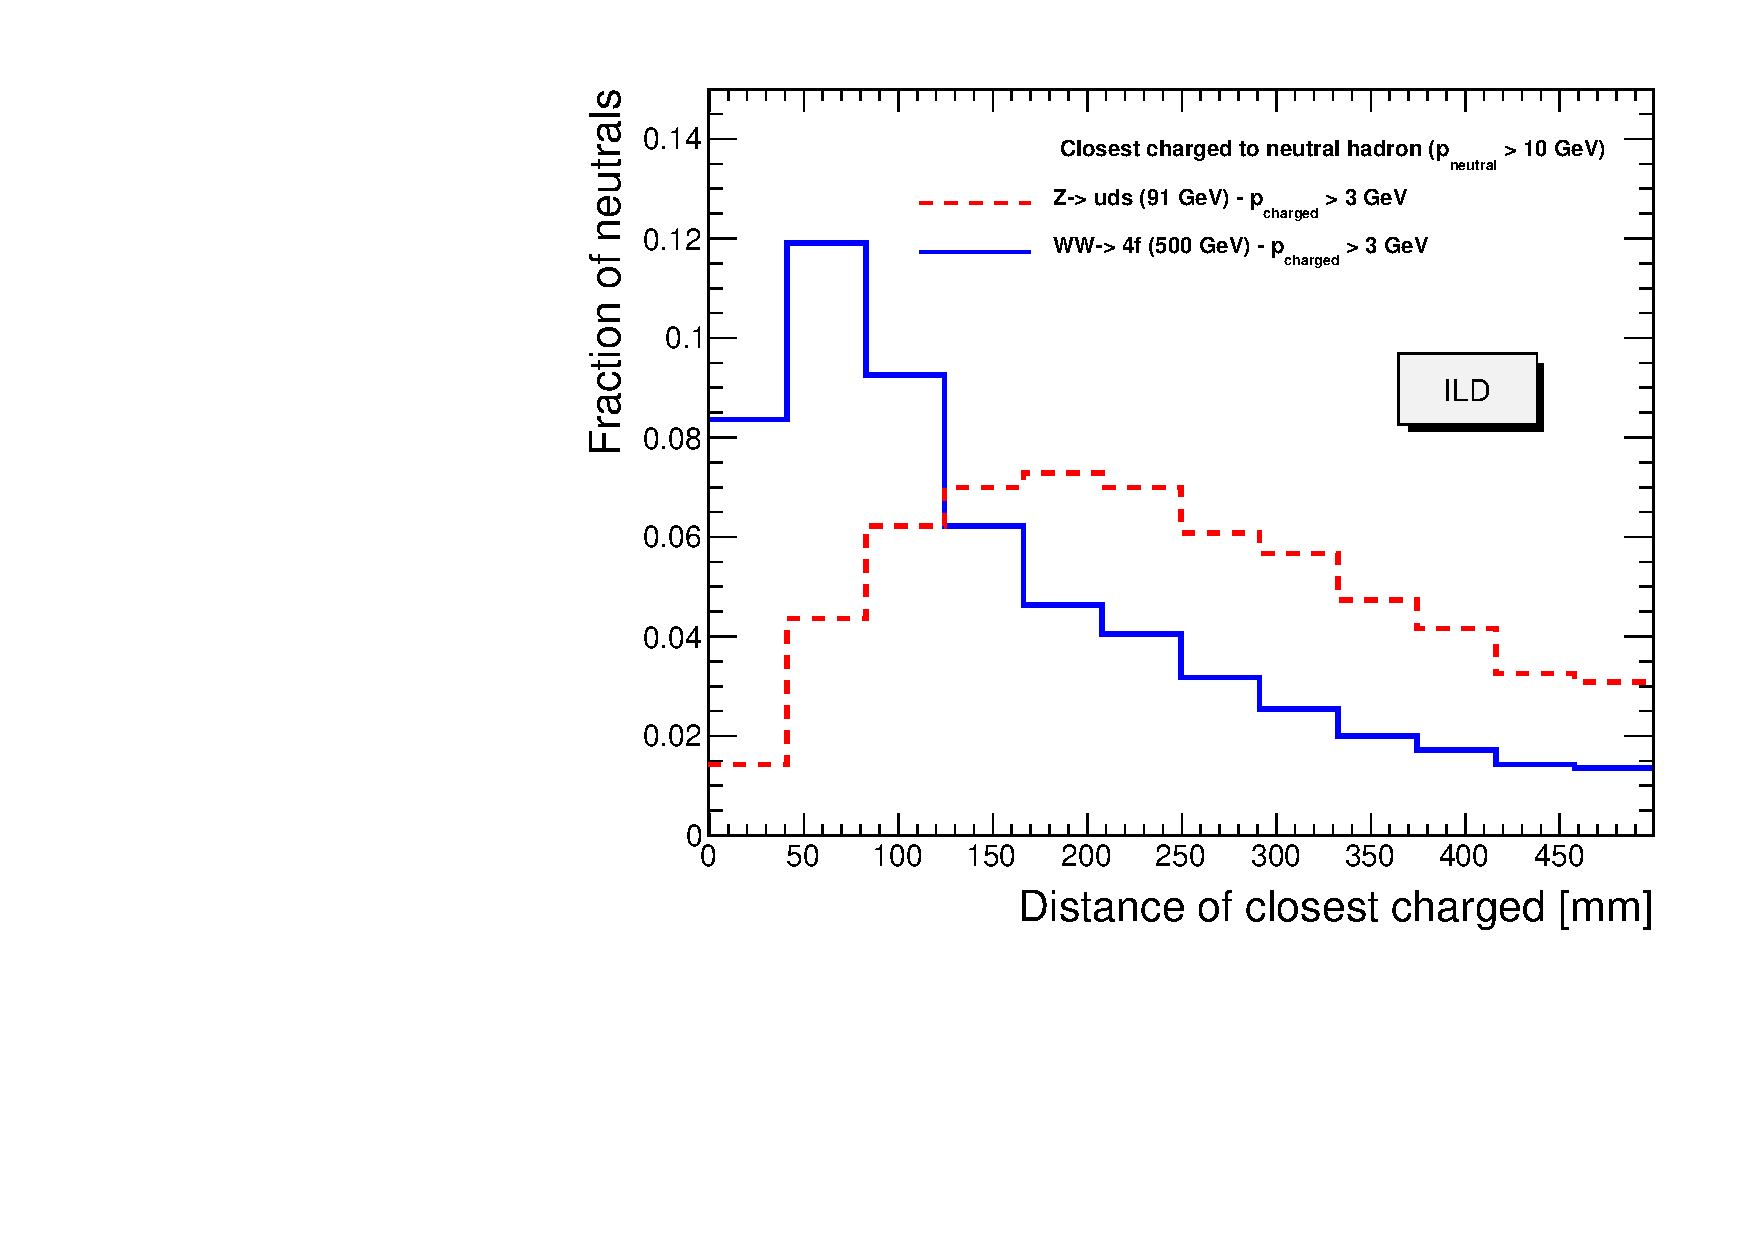
\includegraphics[width=1\linewidth]{../Thesis_Plots/ILD/Stackall_dmin_3GeVneu_10GeVcharged_final_3_morestat.pdf}
    \caption{} \label{fig:distancefrontfacejets}
  \end{subfigure}
  \caption{\subref{fig:momentumparticlejets}) Momentum distribution for charged particles in simulated \ee{}\ra{} \Zqq{} with $q = u,d,s$ at \rts{} = 91 \GeV and \ee{}\ra{} \WWqqqq{} where q is a quark at \rts{} = 500 \GeV. \subref{fig:distancefrontfacejets}) Distribution of distances to the closest charged track for neutral particles produced in \Zqq{} and \WWqqqq{} processes measured at the front face of the electromagnetic calorimeter in the ILD detector.} \label{fig:Motivation}
\end{figure}

In this section, the effect of timing cuts on hadronic showers is investigated. The study was performed using the \ilcsoft framework for reconstruction. In order to study the effect of timing on hadronic shower properties, the initial study was performed assuming a perfect timing resolution (i.e. the timing information is the Monte-Carlo truth). In a following step, several timing resolutions were used to assess different scenarios.

\subsection{Event Selection}

In this analysis, events are selected similar as in \cite{SoftCompNew2012} and based on the following criteria:
\begin{itemize}
  \item A single Particle Flow Object (PFO) is reconstructed (except for section \ref{sec:ImpactNPFO}).
  \item The reconstructed particle must be in the barrel region such as $|\cos\theta| < 0.7$.
  \item The ratio of $E_{ECAL}/E_{total}$ is under 5\% to ensure that the shower is mostly in the HCAL.
  \item The start of the shower must be inside the first 5 HCAL layers in order to have the shower mostly in the HCAL and reduce the effect of leakage.
\end{itemize}

In the following analysis, the timing cut is defined such as the calorimeter hits are rejected if $t_{hit} - t_{ToF} > t_{cut}$ (see section \ref{subsec:ILDDigiCalo} for the definition of $t_{hit}$ and $t_{ToF}$).

\subsection{Impact of timing cuts on Particle Flow Object reconstruction}
\label{sec:ImpactNPFO}

Firstly, the impact of timing cuts on the number of reconstructed particles was investigated. The figure \ref{fig:DistriPFO} shows the number of reconstructed PFO per event for different timing cuts. The figure shows that up to four, five PFOs can be reconstructed in a single event. These events are primarily due to small shower fragments that are not correctly associated to the main cluster. In addition, the figure demonstrates that timing cuts reduces the number of events reconstructed with more than one PFO. It is expected because timing cuts would likely remove shower fragments that are not associated to the main cluster and therefore reconstruct less events with more than one PFO. Furthermore, the impact has been studied for all energies between 5 GeV and 90 GeV. Figure \ref{fig:EventRecoPFO} shows the number of events reconstructed with a single PFO relative to the default configuration with 100 ns timing cut. Timing cuts increase the fraction of reconstructed events containing a single PFO over all energies between 10-25\%.

\begin{figure}[htbp!]
  \centering
  \begin{subfigure}[t]{0.49\textwidth}
    \centering
    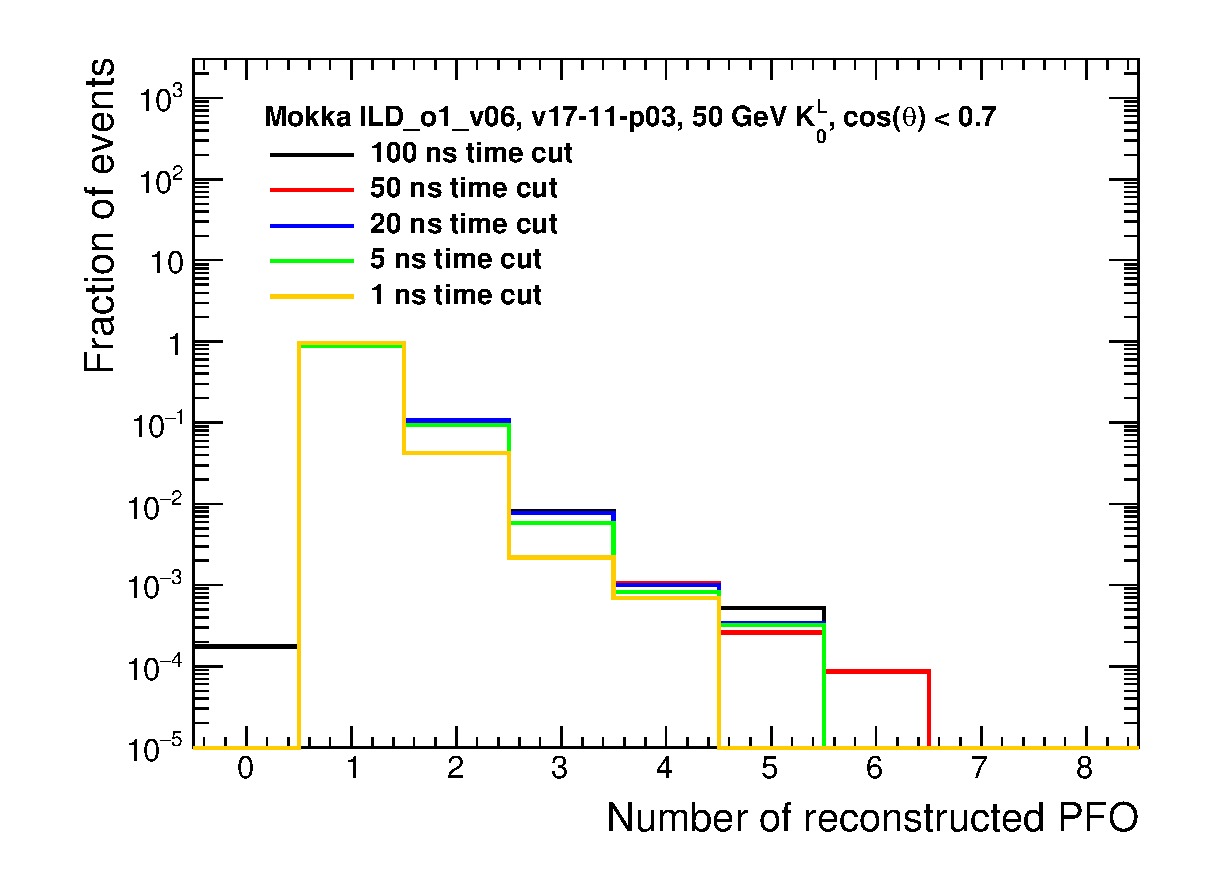
\includegraphics[width=1\linewidth]{../Thesis_Plots/ILD/AdditionalPlots/Plots/NumberReconstructedPFO_TimeCuts_50GeV.eps}
    \caption{} \label{fig:DistriPFO}
  \end{subfigure}
  \hfill
  \begin{subfigure}[t]{0.49\textwidth}
    \centering
    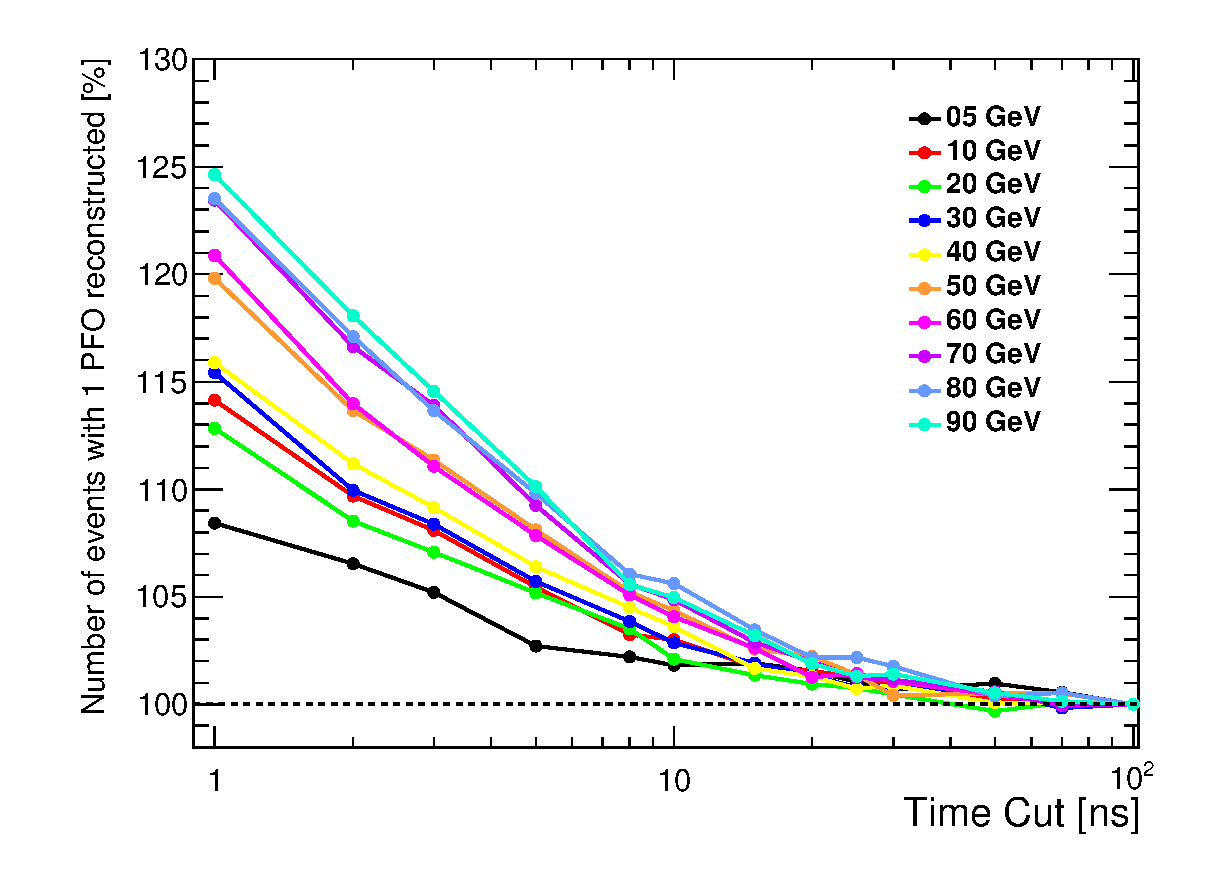
\includegraphics[width=1\linewidth]{../Thesis_Plots/ILD/NoSmearing/Plots/NumberEvents_PFO_TimeCuts_noSmearing.eps}
    \caption{} \label{fig:EventRecoPFO}
  \end{subfigure}
  \caption{\subref{fig:DistriPFO}) Distribution of the number of PFO reconstructed per event for 50 GeV \kzeroL{} in the ILD barrel for different timing cuts. It shows that timing cuts indeed improves the number of events reconstructed with a single PFO but as well a large tail is present. The use of timing cuts reduces slightly the tail of the distribution. \subref{fig:EventRecoPFO}) Number of events reconstructed with only a single PFO normalized to the number of events in the case of 100 ns. It shows a relative increase with a lower timing cut, up to 10-25\% more events are reconstructed with a single PFO using a 1 ns timing cut.}
\end{figure}

To understand more into details what happens, the figures \ref{fig:Energy2ndCluster} and \ref{fig:Distance2ndCluster} show the energy distribution and the distance of the second most energetic cluster to the main cluster for events where more than one PFO is reconstructed for 50 GeV \kzeroL{} for different timing cuts of 100 ns and 1 ns.

\begin{figure}[htbp!]
  \centering
  \begin{subfigure}[t]{0.49\textwidth}
    \centering
    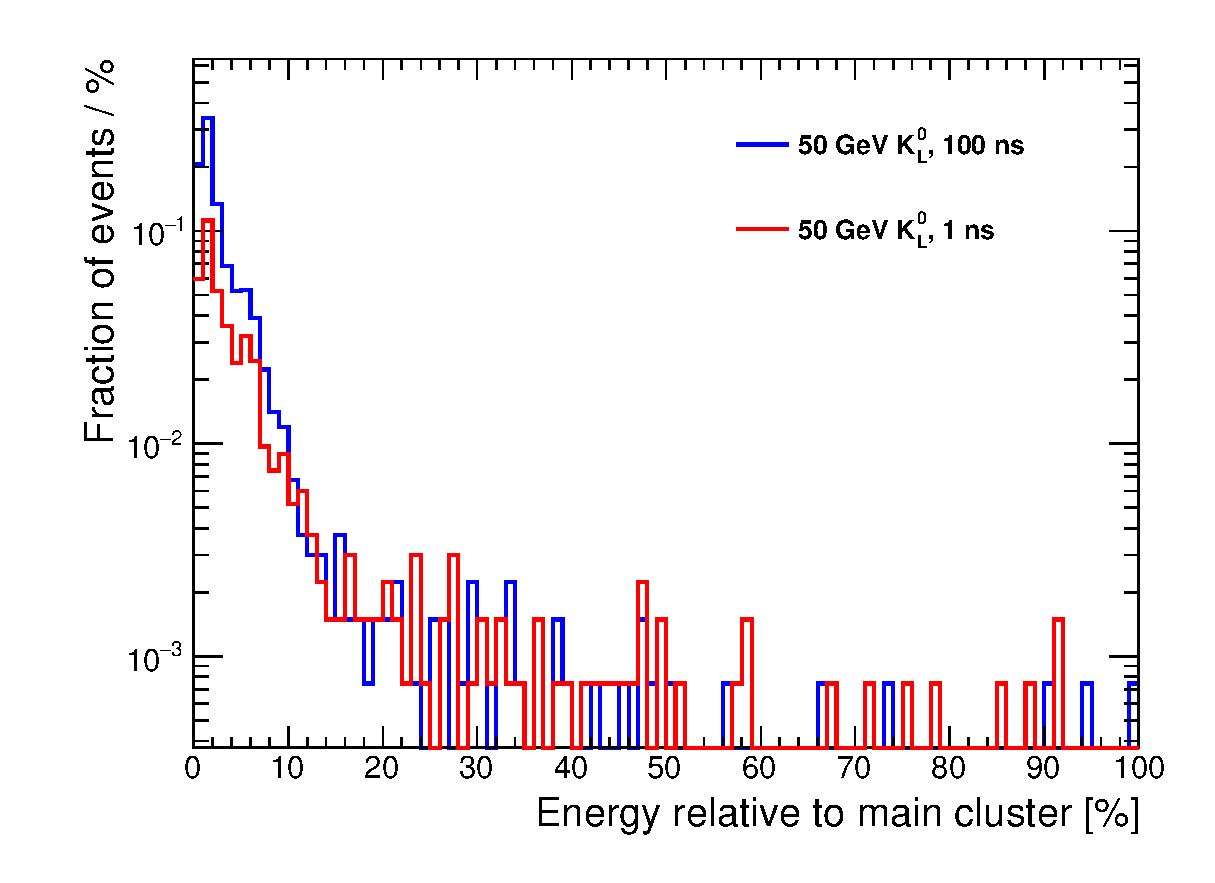
\includegraphics[width=1\linewidth]{../Thesis_Plots/ILD/AdditionalPlots/Plots/Energy2ndCluster_100ns_50GeV.eps}
    \caption{} \label{fig:Energy2ndCluster}
  \end{subfigure}
  \hfill
  \begin{subfigure}[t]{0.49\textwidth}
    \centering
    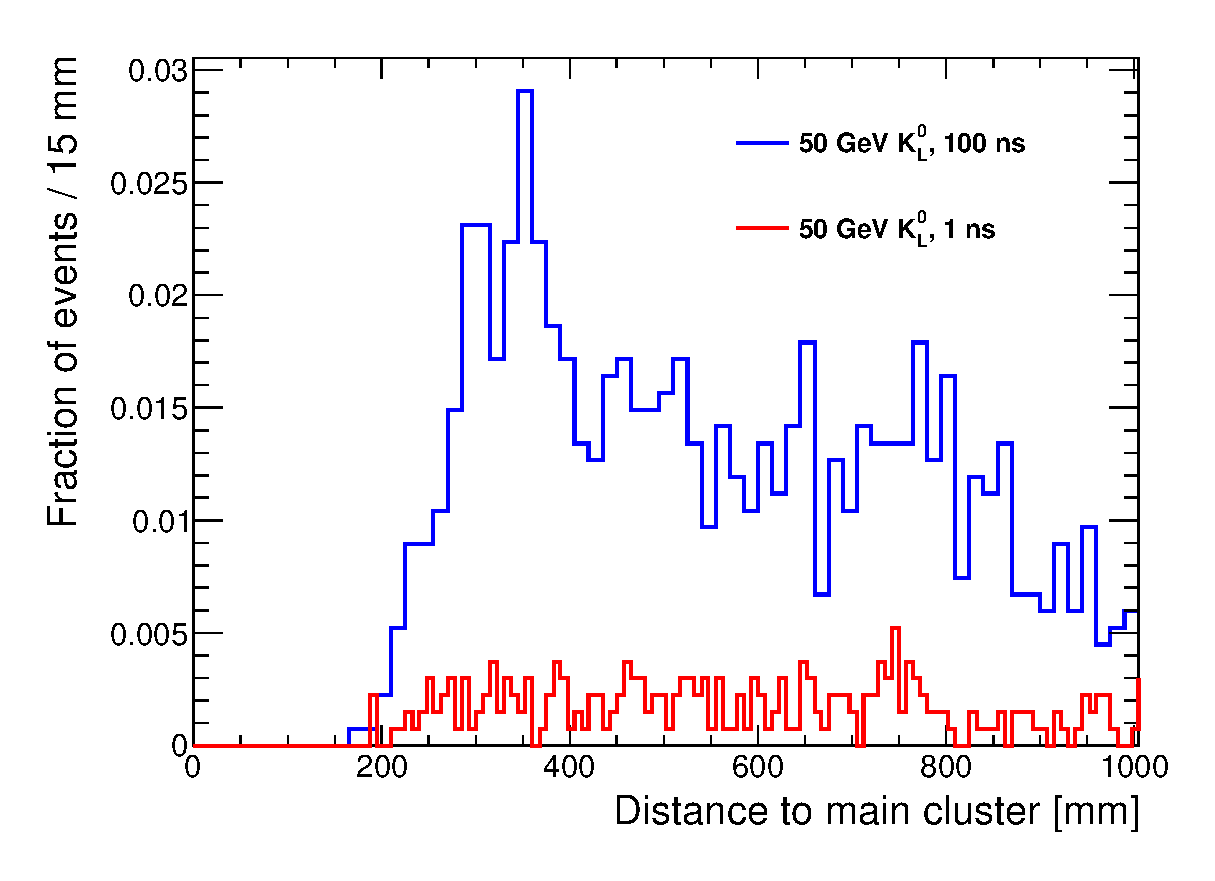
\includegraphics[width=1\linewidth]{../Thesis_Plots/ILD/AdditionalPlots/Plots/Distance2ndCluster_100ns_50GeV.eps}
    \caption{} \label{fig:Distance2ndCluster}
  \end{subfigure}
  \caption{\subref{fig:Energy2ndCluster}) Normalized energy distribution of 2$^{nd}$ most energetic cluster. One can see that most of the entries are below few percents. \subref{fig:Distance2ndCluster}) Normalized distance to main PFO of 2$^{nd}$ most energetic cluster. The distribution peaks in the region 25-30 cm.}
\end{figure}

The figures show that the second most energetic cluster has mostly an energy below few percents of the main cluster energy, over 97\% of the entries are below 20\% of the main cluster energy. The mean distance of this second cluster is around 25-30 cm from the main cluster with around 22\% of entries below 40 cm and is comprised of a long tail to higher distances. This is visible for both timing cuts of 100 ns and 1 ns. This tells us that mainly the split cluster has little energy compared to the main cluster and is situated at around 7 to 10 AHCAL tiles away from the main cluster which is far enough to not be recombined by PandoraPFA with the main cluster. These clusters may be coming from low energy neutrons traveling through the calorimeter. This explains that by introducing a timing cut more events are reconstructed with a single PFO. As shown in chapter \ref{chap:TimingPions}, low energy neutrons are correlated with low energy deposition and late depositions far away from the shower axis and are removed with a timing cut below few tens of nanoseconds.

\subsection{Impact of timing cuts on calorimeter performance and hadronic showers}

\subsubsection{Assuming perfect time resolution}

The following section presents results of timing cuts on the calorimeter performance and hadronic showers assuming a perfect time resolution. To avoid any clustering effects, the study was performed at the calorimeter hit level. The reconstructed energy is obtained by summing up the energy of all hits in the calorimeters. In addition, several shower observables were studied as a function of the timing cut for energies from 5 \GeV to 90 \GeV \kzeroL. The different time cuts used are: 1, 2, 3, 5, 8, 10, 15, 20, 25, 30, 50, 70 and \SI{100}{\nano\second}.

The figures \ref{fig:linearityNoSmearing} and \ref{fig:resoNoSmearing} show the effect of the timing cuts on the calorimeter response and energy resolution. The response decreases and energy resolution gets degraded for lower timing cuts. The response degrades as much as 10\% at high energies for a 1 ns timing cut. This would effectively mean that with a harder timing cut, more hits of the shower are removed but without affecting much the total shower energy.

\begin{figure}[htbp!]
  \centering
  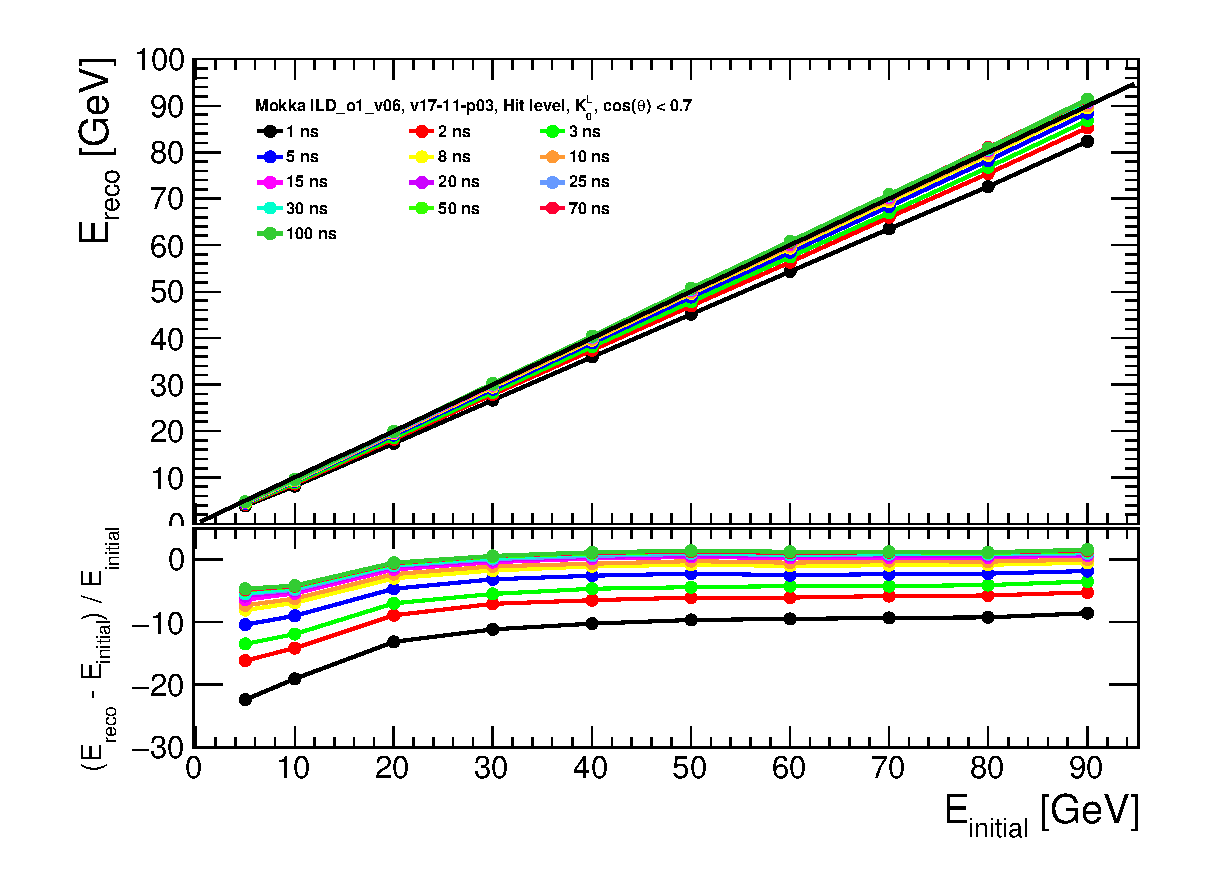
\includegraphics[width=0.6\linewidth]{../Thesis_Plots/ILD/NoSmearing/Plots/Linearity_TimeCuts_noSmearing.eps}
  \caption{The top plot shows the reconstructed energy $E_{reco}$ as a function of the initial particle energy $E_{initial}$ for different timing cuts assuming a perfect time resolution. The bottom plot represent the relative deviation to the line $x=y$ for the different time cuts.} \label{fig:linearityNoSmearing}
\end{figure}

The figure \ref{fig:resoNoSmearing} shows the relative impact on the calorimeter energy resolution as a function of the energy for different timing cuts. The energy resolution is very little affected for a cut of above \SI{20}{\nano\second}. Then for a cut under \SI{20}{\nano\second}, the resolution starts to degrade slowly relatively in the same way for all energies. A hard cut of 1 ns will degrade greatly the energy resolution by around 20-30\% relative to 100 ns. The degradation of the energy resolution comes mostly from an increase of the constant term. Naively, ones would expect that if for example randomly 10\% of the shower energy is removed in average that then the resolution would behave as $\sqrt{E}$ and would degrade by around 6\% from a statistical point of view. However, timing cuts do not remove hits randomly. There is a bias to remove late hits which are mostly coming from the hadronic component of the shower. As in hadronic showers, the electromagnetic and hadronic fraction of the shower is fluctuating a lot on an event-by-event basis this may affect the energy resolution much more. To understand this effect, a similar study as in \cite{SoftCompNew2012} has been performed in section \ref{sec:eresdegrad}. The figure \ref{fig:ShowerEnergyNoSmearing} shows the fraction of energy of the shower as a function of the timing cut. It shows that 99\% of the shower energy is deposited within 15 ns. Thus, up to a timing cut of around 15 ns, the energy resolution should not be degraded which is compatible with the observation in figure \ref{fig:resoNoSmearing}.

\begin{figure}[htbp!]
  \centering
  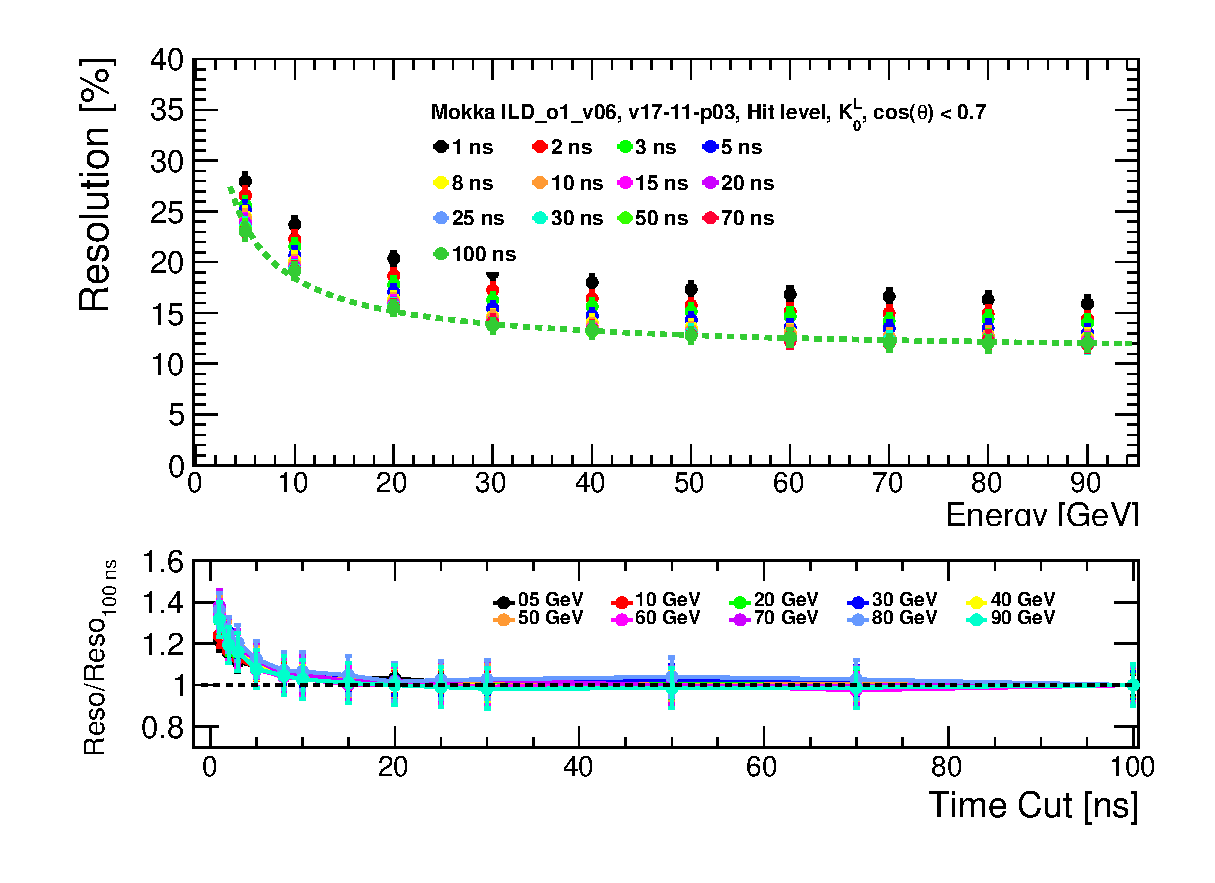
\includegraphics[width=0.6\linewidth]{../Thesis_Plots/ILD/NoSmearing/Plots/ShowerResoAbsolute_TimeCuts_noSmearing.eps}
  \caption{The top plot illustrates the relative energy resolution ($\frac{\sigma_{E}}{E}$) at single particle level for different timing cuts. The green line is a fit performed at \SI{100}{\nano\second} of the form $\frac{\sigma_{E}}{E} = \frac{a}{\sqrt{E}} \bigoplus b$ where $a$ is the stochastic term ($46.73\% \pm 2.03$) and $b$ the constant term ($10.99\% \pm 0.41$). The bottom plot shows the relative change of the energy resolution compared to \SI{100}{\nano\second} as function of the timing cut for each particle energy. The error bars represent the statistical uncertainty.} \label{fig:resoNoSmearing}
\end{figure}

\begin{figure}[htbp!]
  \centering
  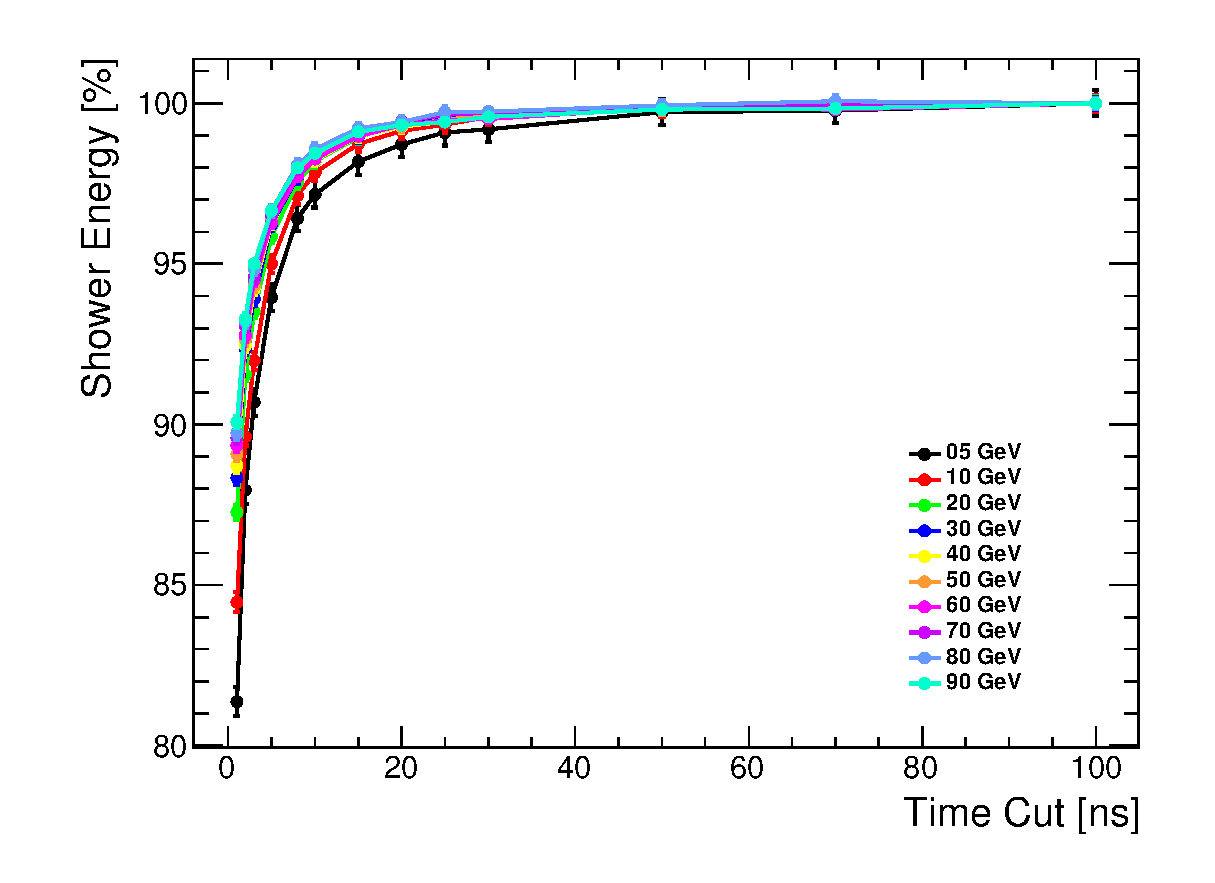
\includegraphics[width=0.6\linewidth]{../Thesis_Plots/ILD/NoSmearing/Plots/ShowerEnergy_TimeCuts_noSmearing.eps}
  \caption{Fraction of the total shower energy as a function of the timing cut. The fraction is defined such as the shower energy at a 100 ns timing cut is 100\%.} \label{fig:ShowerEnergyNoSmearing}
\end{figure}

The figure \ref{fig:RadialProfNoSmearing} shows a \kzeroL{} radial shower profile at 50 GeV. For the calculation of the radial profile, the energy within each radial bin of 3 cm width is summed up and normalized to the bin area. The average energy deposit per area is displayed as a function of the distance to the shower main axis. Almost all the shower energy is contained in a circle of few centimeter radius. The influence of timing cuts is highly visible in the tail of the distribution corresponding to the halo of the shower while they have little influence on the energy deposited in the core of the shower. A cut at 1 ns reduces up to 30\% the radial shower profile above 30-40 cm. In addition, an increase of energy in the two first bins of the distribution is visible. This effect is related to a displacement of the center of gravity as function of the timing cut because outer hits of the shower are removed. This was verified by calculating the distance relative to a fixed reference, i.e the endpoint of the MC particle, instead of the center of gravity. In this case, it has been observed that timing cuts remove only part of the distribution tail without affecting the two first bin of the distribution.

\begin{figure}[htbp!]
  \centering
  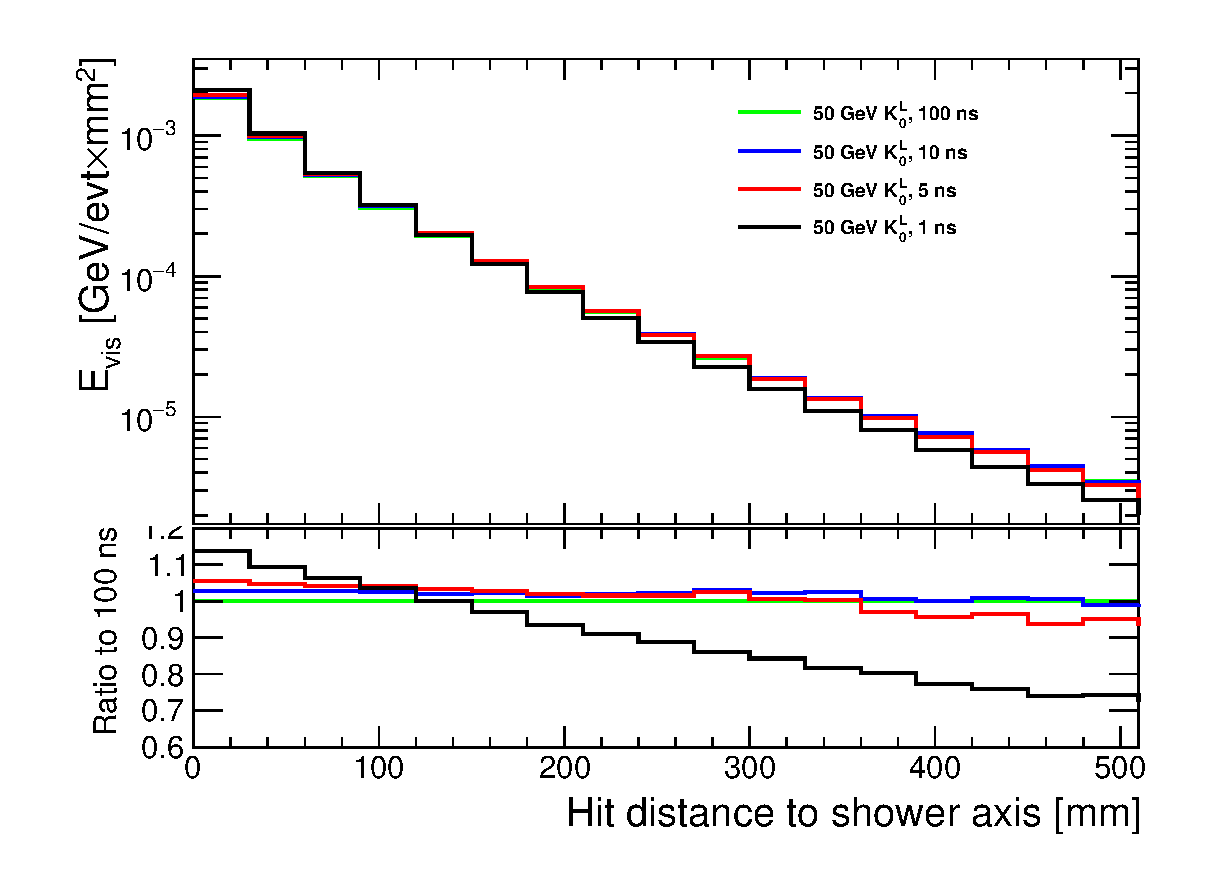
\includegraphics[width=0.6\linewidth]{../Thesis_Plots/ILD/NoSmearing/Plots/RadialProfileOverlay_noSmearing.eps}
  \caption{The top plot shows the radial profile of a 50 \GeV hadronic shower overlaid for different timing cuts. The bottom plot shows the ratio of the histograms to \SI{100}{\nano\second} radial profile.} \label{fig:RadialProfNoSmearing}
\end{figure}

The shower width is calculated as the mean distance of all the hits to the shower main axis according to the formula:
\begin{equation}
  w = \sqrt{\frac{\Sigma_i E_i \times r_i^2}{\Sigma_i E_i}}
\end{equation}
where $E_i$ is the energy of the i-th hit and $r_i$ is the distance of the i-th hit to the cluster main axis.

The figures \ref{fig:ShowerWidthNoSmearing} and \ref{fig:ShowerWidthAbsoNoSmearing} show the shower width for different particle energies as function of the timing cut. It shows that a timing cut of \SI{1}{\nano\second} can reduce the shower width by around 40-50\%. One can observe also that the shower width at 5 and 10 \GeV are behaving differently than for higher energies. This may come from the transition from the Bertini model (BERT) to the quark string gluon model (QGSP) in the physics list in this energy range. Looking at the shower width in absolute value, hadronic showers are slightly wider at lower energies with a mean width of $\sim$\SI{125}{\milli\meter} for 10 GeV and $\sim$\SI{115}{\milli\meter} for 90 GeV. This may be related to the fact that the electromagnetic fraction in a hadronic shower increases with energy. Therefore, the mean shower width is reduced because the hits close to the shower axis carry most of the energy. In general, all energies behave in a rather similar manner.

\begin{figure}[htbp!]
  \centering
  \begin{subfigure}[t]{0.49\textwidth}
    \centering
    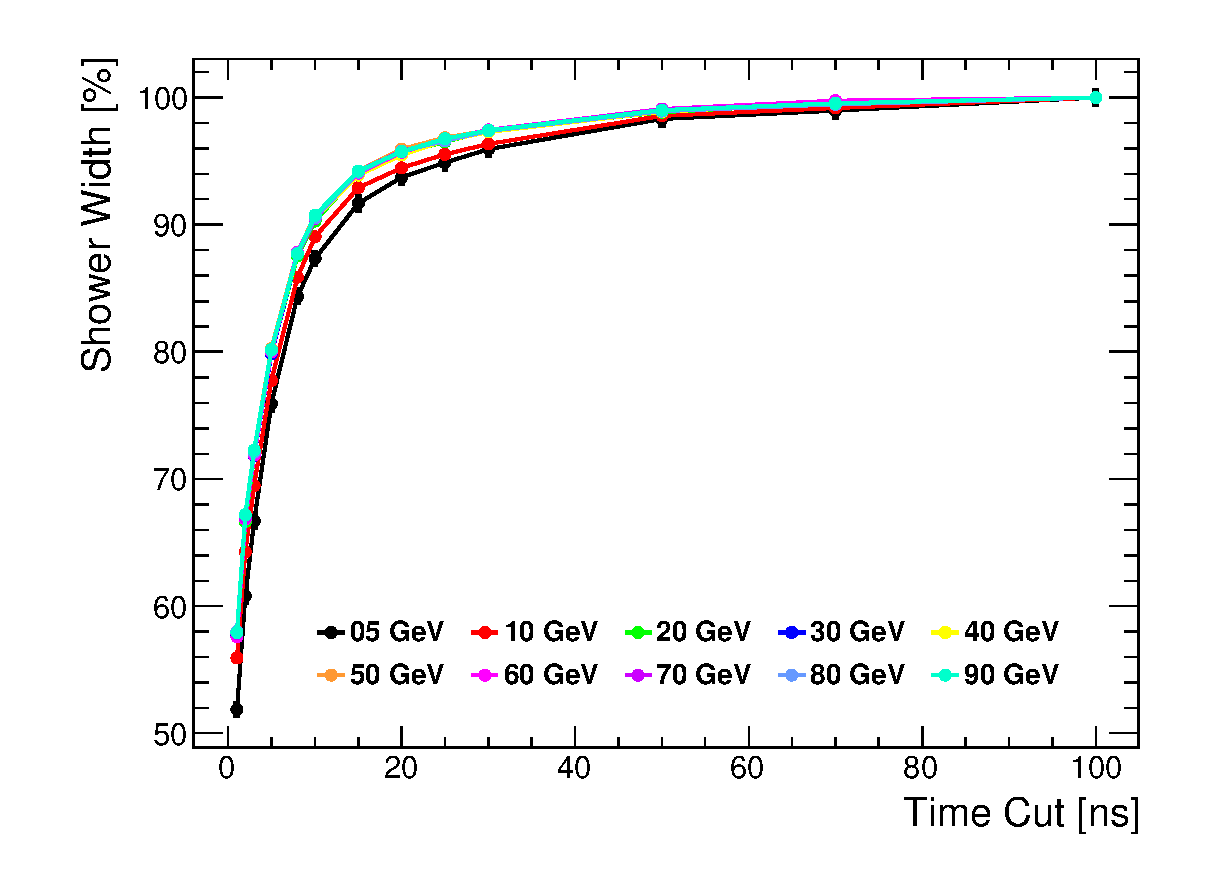
\includegraphics[width=1\linewidth]{../Thesis_Plots/ILD/NoSmearing/Plots/ShowerWidth_TimeCuts_noSmearing.eps}
    \caption{} \label{fig:ShowerWidthNoSmearing}
  \end{subfigure}
  \hfill
  \begin{subfigure}[t]{0.49\textwidth}
    \centering
    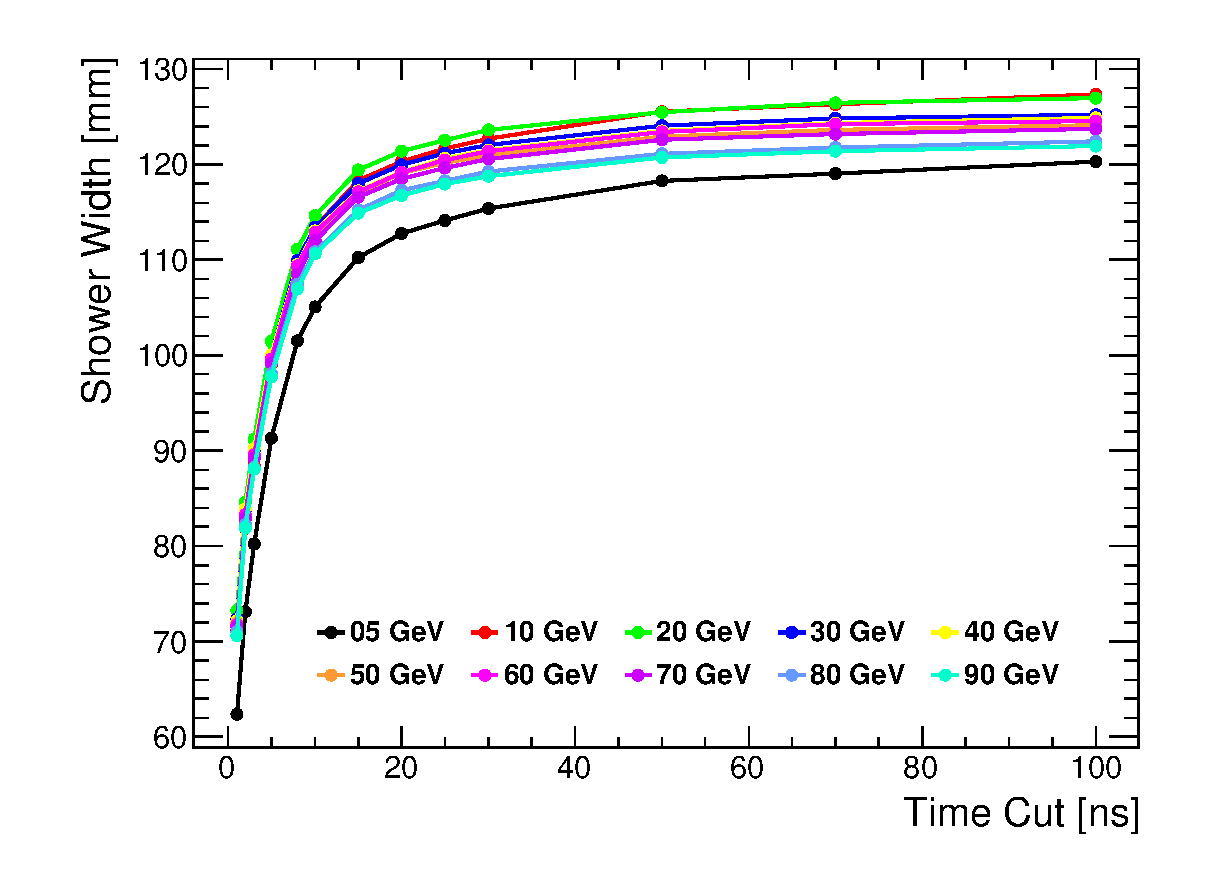
\includegraphics[width=1\linewidth]{../Thesis_Plots/ILD/NoSmearing/Plots/ShowerWidthAbso_TimeCuts_noSmearing.eps}
    \caption{} \label{fig:ShowerWidthAbsoNoSmearing}
  \end{subfigure}
  \caption{\subref{fig:ShowerWidthNoSmearing}) Mean shower width as a function of the timing cut for different \kzeroL{} energies between 5 GeV and 90 GeV. The y-axis has been normalized to the shower width at \SI{100}{\nano\second}. The shower width decreases steadily as a function of the timing cut, indicating that the shower gets narrower. \subref{fig:ShowerWidthAbsoNoSmearing}) Mean shower width in \SI{}{\milli\meter} as a function of the timing cut for different \kzeroL{} energies between 5 GeV and 90 GeV. Under \SI{20}{\nano\second}, the shower width is very similar indicating the core of the shower is fairly identical for all energies.}
\end{figure}

Finally, it is interesting to look at the gain in the reduction of the shower width compared to the loss in energy resolution. Reducing the shower width by applying timing cuts could help to improve the pattern recognition in PandoraPFA. The figure \ref{fig:ShowerWidthResoNoSmearing} shows the resolution loss as a function of the shower width for different \kzeroL{} energies and different timing cuts. The bottom plot shows that the gain in shower width is behaving in the same way for all energies. The shower width is reduced and the resolution gets slowly degraded for tighter timing cuts. The main point here is that the gain in shower width is great, up to 40\% decrease in shower width, compared to the loss in energy resolution which is around 4-6\% (absolute) that could be recovered in a next step after pattern recognition.

\begin{figure}[htbp!]
  \centering
  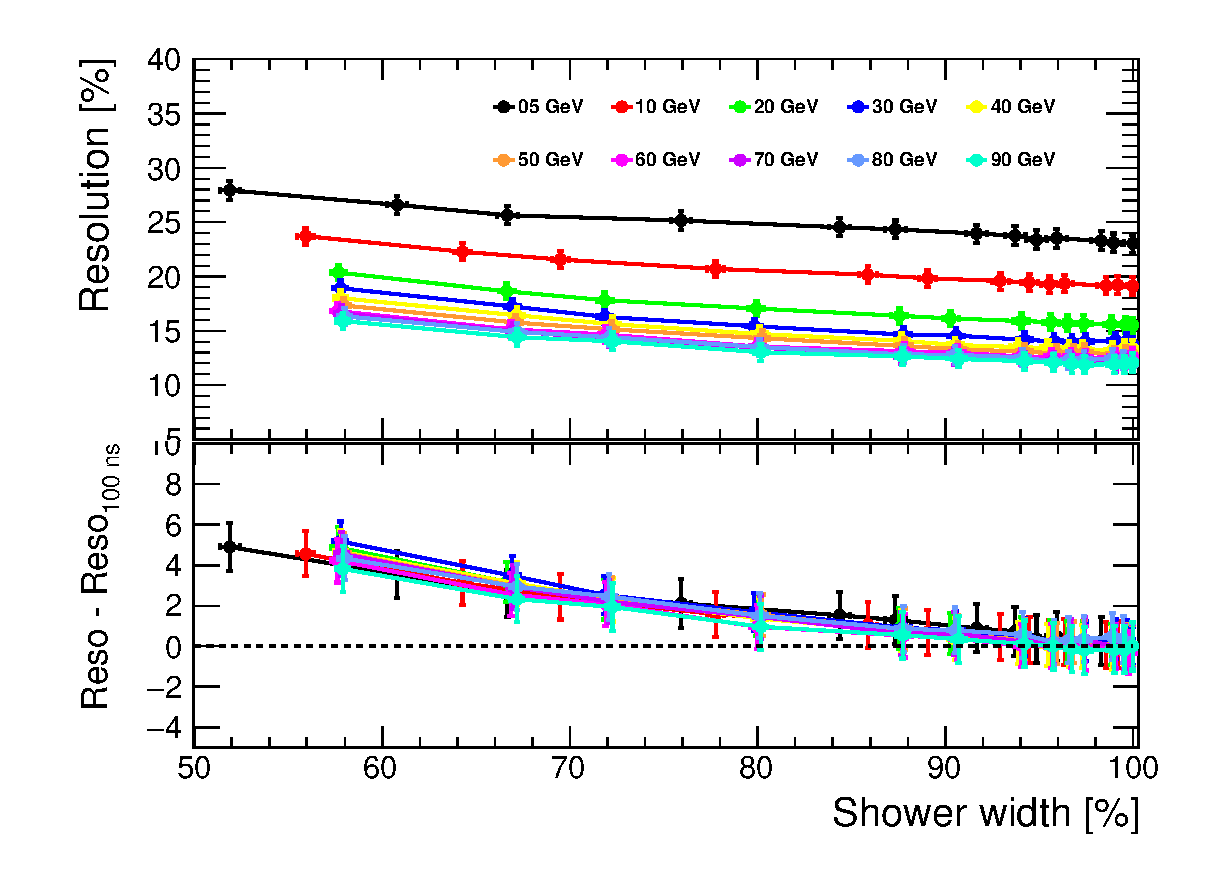
\includegraphics[width=0.6\linewidth]{../Thesis_Plots/ILD/NoSmearing/Plots/ShowerWidth_Resolution_noSmearing.eps}
  \caption{The top plot shows the energy resolution as a function of the relative shower width for different particle energies. Each point represents a timing cut from \SI{1}{\nano\second} ns to \SI{100}{\nano\second} from left to right. The bottom plot shows the absolute loss of resolution as a function of the relative shower width.} \label{fig:ShowerWidthResoNoSmearing}
\end{figure}

To conclude, this study shows that the use of timing cuts give a great advantage in order to improve pattern recognition without degrading too much the energy resolution of a hadronic shower. A timing cut up to 15 ns does not degrade the energy resolution and would reduce the shower width by around 10\%. A cut below 15 ns starts to degrade heavily the energy resolution and reduce as well the shower width. The needed time resolution depends on the aim for the use of timing. A cut at 25 ns like the LHC look good enough. However, in order to locate the electromagnetic core of the shower, a much lower timing cut is needed thus the time resolution must be better. This study assumes a perfect timing resolution which does not reflect the reality. In the next section, different time resolutions were assumed based on the current knowledge on the timing resolution of the foreseen front-end electronics.

\subsubsection{In a realistic scenario}
\label{sec:RealisticScenario}

In this section, a similar study is performed as in previous section \ref{sec:MCLevelILDTiming}. Instead, it assumes realistic time resolutions based on the current electronic technology. The table \ref{table:TimeReso} sums up the investigated time resolutions. The same selection is applied as in the previous section.

\begin{table}[htb!]
  \centering
  \caption{Assumption on the time resolution of the front-end electronics for different scenarios.} \label{table:TimeReso}
  \begin{tabular}{@{} lc @{}}
    \toprule
    Scenario & Time resolution (ns) \\
    \midrule
    Testbeam & 8 \\
    Scenario 1 & 1 \\
    Scenario 2 & 0.4 \\
    \bottomrule
  \end{tabular}
\end{table}

The testbeam resolution is the time resolution obtained with the current AHCAL technological prototype as shown in section \ref{subsec:Electron_Final}. The Scenario 1 is an assumption on the ideal time resolution which is in the order of the timescale of the development of hadronic showers therefore around 1 ns. And finally, the Scenario 2 is the time resolution which is obtained by assuming a linear extrapolation from the testbeam time resolution by using a faster slow clock of \SI{5}{\mega\hertz} instead of \SI{250}{\kilo\hertz} (20 times faster) although this is probably an optimistic scenario.

Looking at the impact on calorimeter response and energy resolution, the figures \ref{fig:Lin0.4ns} and \ref{fig:Reso0.4ns} show that a time resolution in the order of sub-nanosecond does not affect much the response and energy resolution. The figures \ref{fig:Lin1ns} and \ref{fig:Reso1ns} show that for a time resolution in the nanosecond order, the response and energy resolution does not get affected much also. However, for a cut below 1-2 ns, it will start to degrade the response rapidly, up to 35-40\%. The resolution gets affected as well up to 35-50\% (relative to 100 ns). The figures \ref{fig:Lin8ns} and \ref{fig:Reso8ns} show that for the 8 ns timing resolution, the response and resolution get heavily degraded for timing cuts below 10-20 \SI{}{\nano\second}, up to 55-60\% for the response and around 50-60\% (relative to 100 ns) for the energy resolution.

\begin{figure}[htbp!]
  \centering
  \begin{subfigure}[t]{0.49\textwidth}
    \centering
    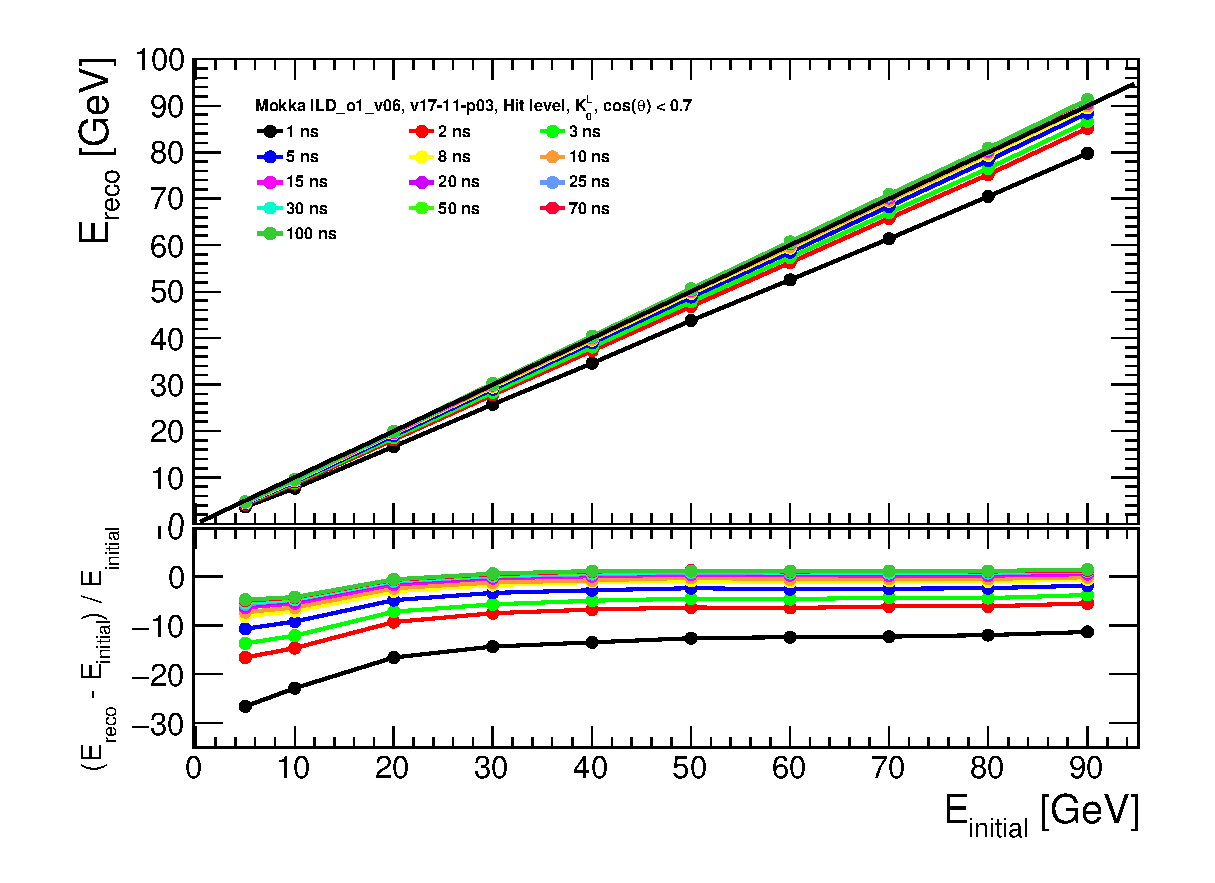
\includegraphics[width=1\linewidth]{../Thesis_Plots/ILD/Smearing_0.4ns/Plots/Linearity_TimeCuts_Smearing1.eps}
    \caption{} \label{fig:Lin0.4ns}
  \end{subfigure}
  \hfill
  \begin{subfigure}[t]{0.49\textwidth}
    \centering
    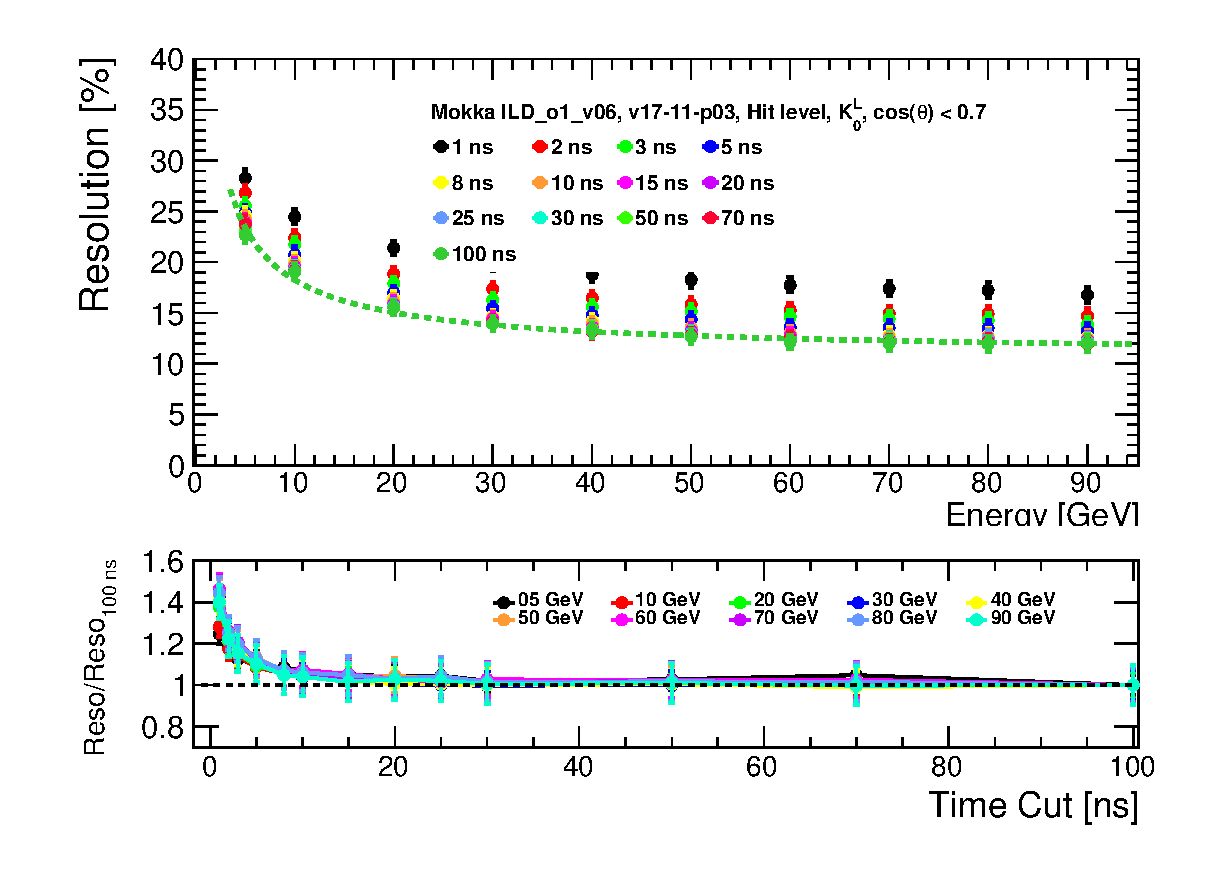
\includegraphics[width=1\linewidth]{../Thesis_Plots/ILD/Smearing_0.4ns/Plots/ShowerResoAbsolute_TimeCuts_Smearing1.eps}
    \caption{} \label{fig:Reso0.4ns}
  \end{subfigure}
  \caption{\subref{fig:Lin0.4ns}) The top plot shows the reconstructed energy $E_{reco}$ as a function of the initial particle energy $E_{initial}$ for different timing cuts assuming a time resolution of \SI{0.4}{\nano\second}. The bottom plot represent the relative deviation to the line $x=y$ for the different time cuts. \subref{fig:Reso0.4ns}) Energy resolution curves for \SI{0.4}{\nano\second} time resolution. The plot represents the relative energy resolution $\frac{\sigma_{E}}{E}$ for kaons from 5 to 90 \GeV for each timing cut. The green line is a fit applied to 100 ns timing cut of the typical form $\frac{\sigma_{E}}{E} = \frac{a}{\sqrt{E}} \bigoplus b$.}
\end{figure}

\begin{figure}[htbp!]
  \centering
  \begin{subfigure}[t]{0.49\textwidth}
    \centering
    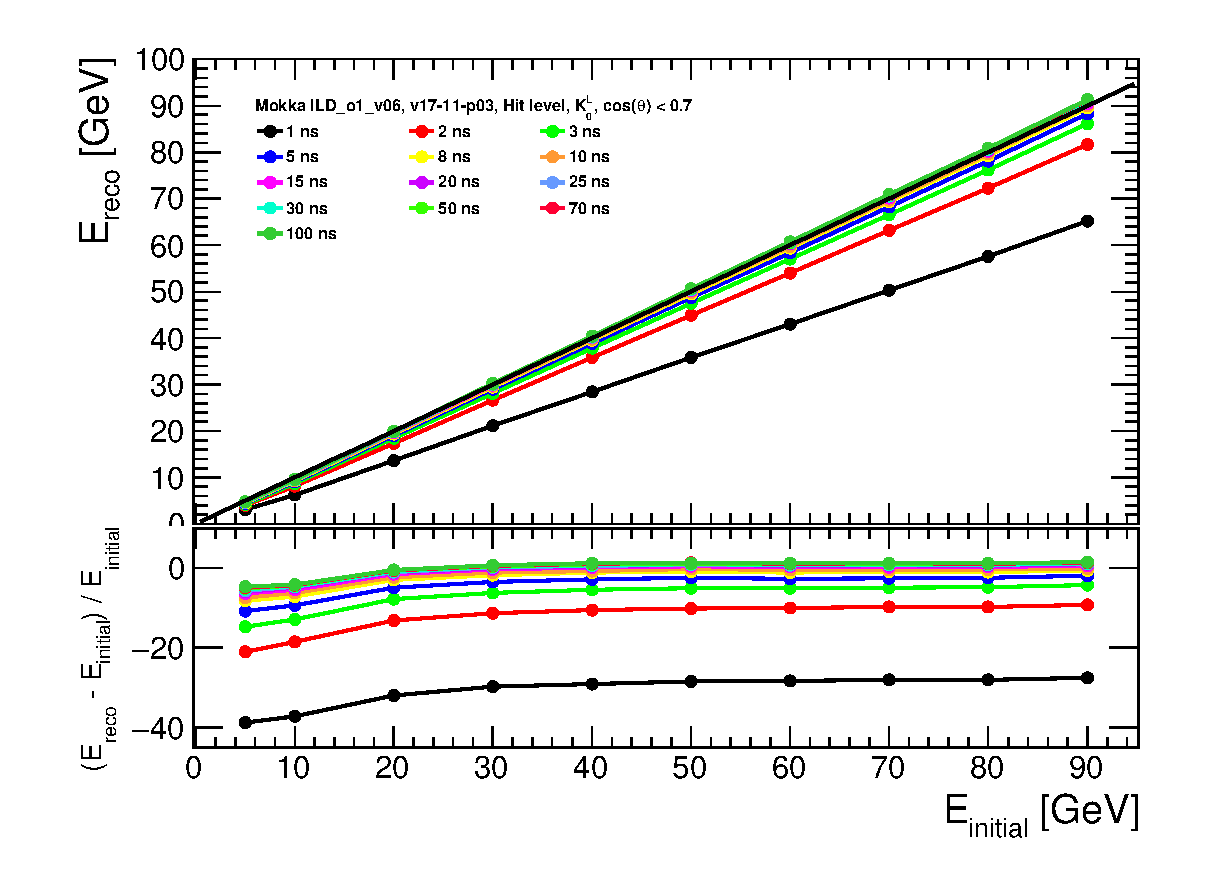
\includegraphics[width=1\linewidth]{../Thesis_Plots/ILD/Smearing_1ns/Plots/Linearity_TimeCuts_Smearing2.eps}
    \caption{} \label{fig:Lin1ns}
  \end{subfigure}
  \hfill
  \begin{subfigure}[t]{0.49\textwidth}
    \centering
    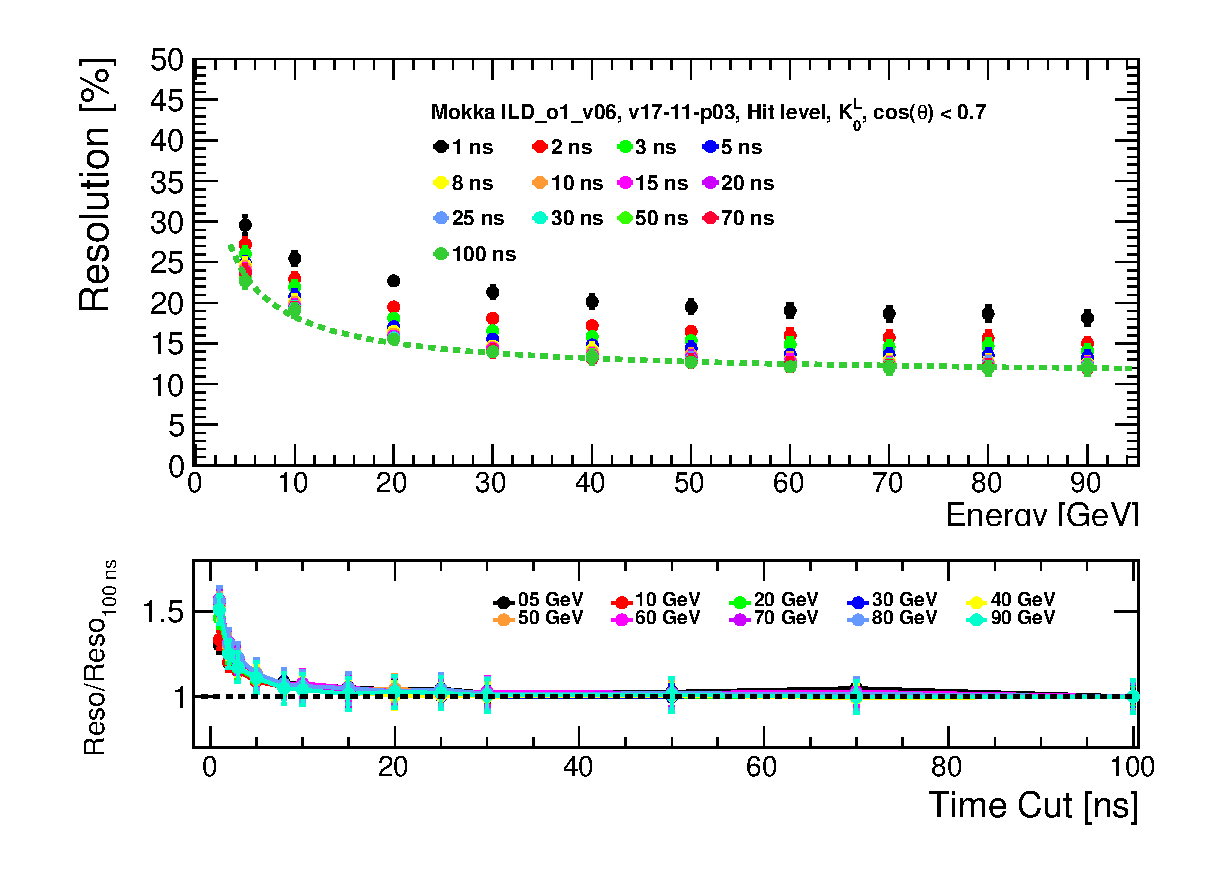
\includegraphics[width=1\linewidth]{../Thesis_Plots/ILD/Smearing_1ns/Plots/ShowerResoAbsolute_TimeCuts_Smearing2.eps}
    \caption{} \label{fig:Reso1ns}
  \end{subfigure}
  \caption{\subref{fig:Lin1ns}) The top plot shows the reconstructed energy $E_{reco}$ as a function of the initial particle energy $E_{initial}$ for different timing cuts assuming a time resolution of \SI{1}{\nano\second}. The bottom plot represent the relative deviation to the line $x=y$ for the different time cuts. \subref{fig:Reso1ns}) Energy resolution curves for \SI{1}{\nano\second} time resolution. The plot represents the relative energy resolution $\frac{\sigma_{E}}{E}$ for kaons from 5 to 90 \GeV for each timing cut. The green line is a fit applied to 100 ns timing cut of the typical form $\frac{\sigma_{E}}{E} = \frac{a}{\sqrt{E}} \bigoplus b$.}
\end{figure}

\begin{figure}[htbp!]
  \centering
  \begin{subfigure}[t]{0.49\textwidth}
    \centering
    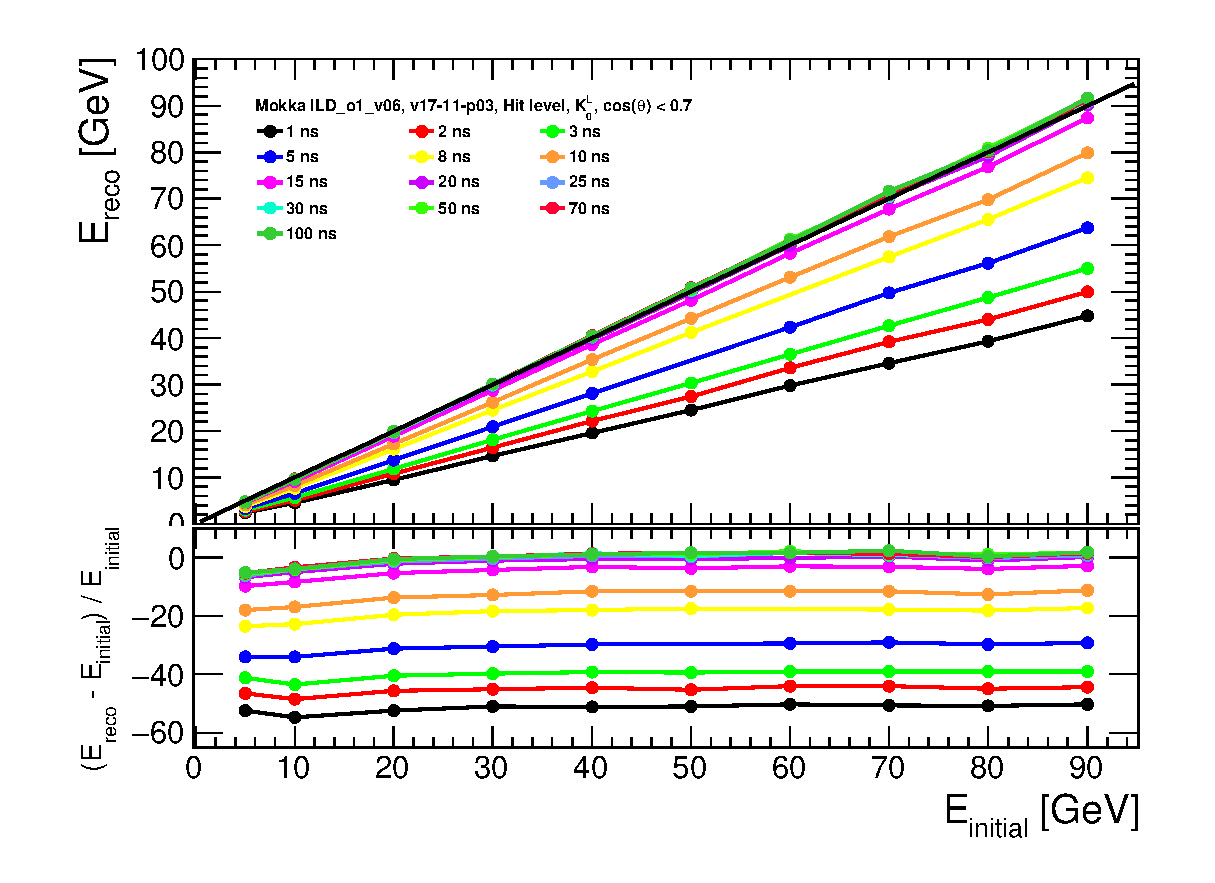
\includegraphics[width=1\linewidth]{../Thesis_Plots/ILD/Smearing_8ns/Plots/Linearity_TimeCuts_Smearing3.eps}
    \caption{} \label{fig:Lin8ns}
  \end{subfigure}
  \hfill
  \begin{subfigure}[t]{0.49\textwidth}
    \centering
    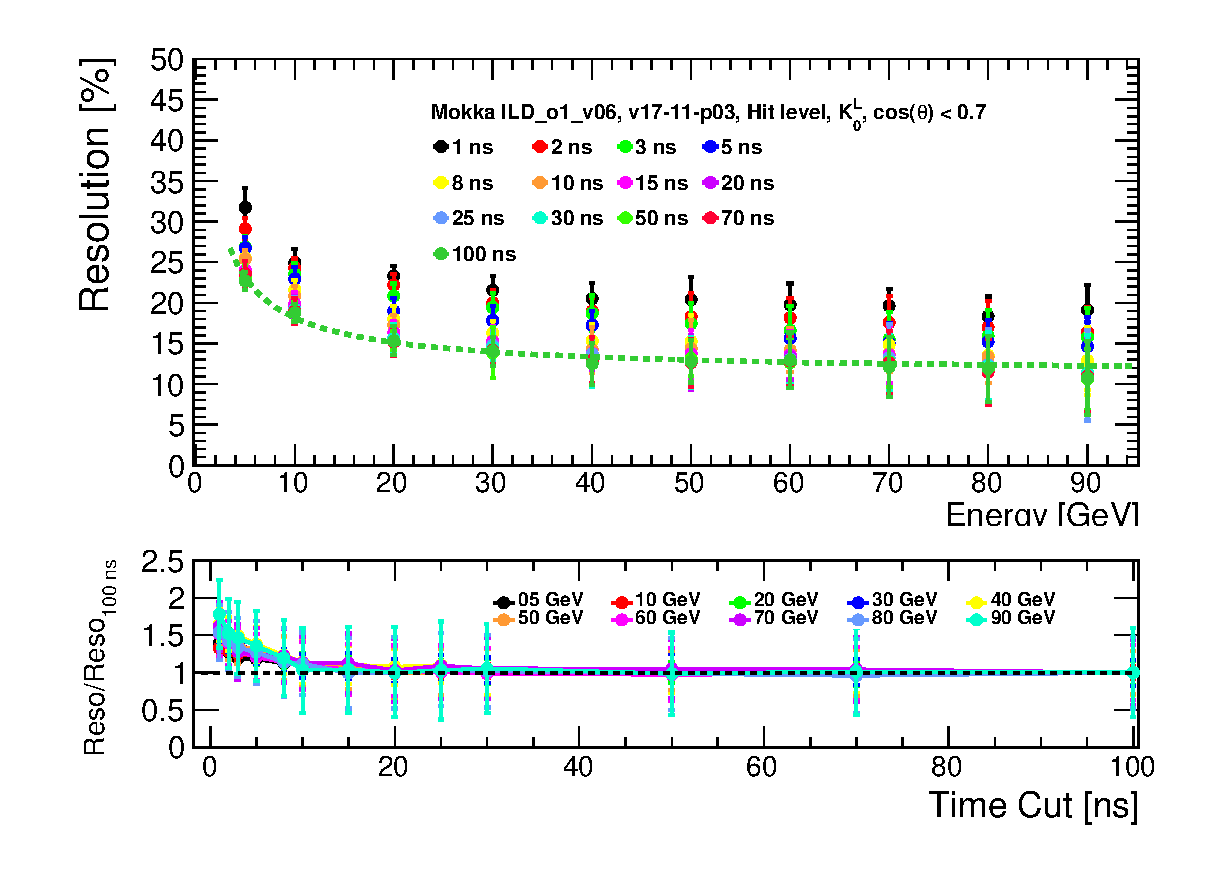
\includegraphics[width=1\linewidth]{../Thesis_Plots/ILD/Smearing_8ns/Plots/ShowerResoAbsolute_TimeCuts_Smearing3.eps}
    \caption{} \label{fig:Reso8ns}
  \end{subfigure}
  \caption{\subref{fig:Lin8ns}) The top plot shows the reconstructed energy $E_{reco}$ as a function of the initial particle energy $E_{initial}$ for different timing cuts assuming a time resolution of \SI{8}{\nano\second}. The bottom plot represent the relative deviation to the line $x=y$ for the different time cuts. \subref{fig:Reso8ns}) Energy resolution curves for \SI{8}{\nano\second} time resolution. The plot represents the relative energy resolution $\frac{\sigma_{E}}{E}$ for kaons from 5 to 90 \GeV for each timing cut. The green line is a fit applied to 100 ns timing cut of the typical form $\frac{\sigma_{E}}{E} = \frac{a}{\sqrt{E}} \bigoplus b$.}
\end{figure}

The energy resolution as a function of the shower width is shown in figures \ref{fig:WidthReso0.4ns}, \ref{fig:WidthReso1ns} and \ref{fig:WidthReso8ns} for different \kzeroL{} energies and different timing cuts assuming the timing resolutions shown in table \ref{table:TimeReso}. In figure \ref{fig:WidthReso0.4ns}, the loss of resolution is comparable when assuming a perfect time resolution while gaining up to 40-50\% in shower width. A sub-nanosecond scale time resolution does not have much impact whatever the timing cut applied. In figure \ref{fig:WidthReso1ns}, the energy resolution gets degraded by around 2\% (absolute) for the same decrease of 40-50\% in shower width. This loss in energy resolution is acceptable even with a tight timing cut and could be recovered in a later stage by adding few hits around the core of the shower to the identified main cluster. In figure \ref{fig:WidthReso8ns}, the same loss in resolution of 2\% (absolute) would only yield a reduction of 30\% in the shower width and corresponds to a timing cut of around 10 ns.

\begin{figure}[htbp!]
  \centering
  \begin{subfigure}[t]{0.6\textwidth}
    \centering
    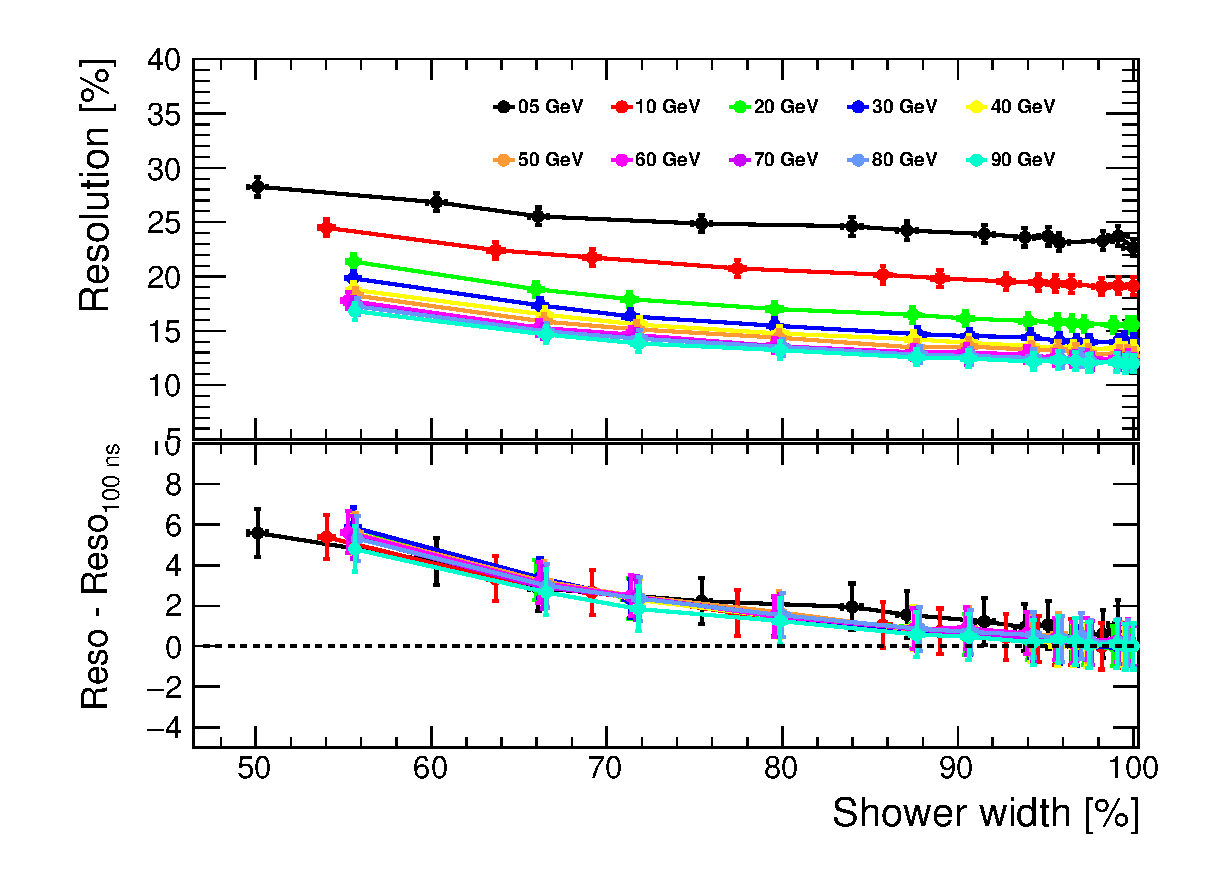
\includegraphics[width=1\linewidth]{../Thesis_Plots/ILD/Smearing_0.4ns/Plots/ShowerWidth_Resolution_Smearing1.eps}
    \caption{\SI{0.4}{\nano\second} time resolution.} \label{fig:WidthReso0.4ns}
  \end{subfigure}
  \begin{subfigure}[t]{0.6\textwidth}
    \centering
    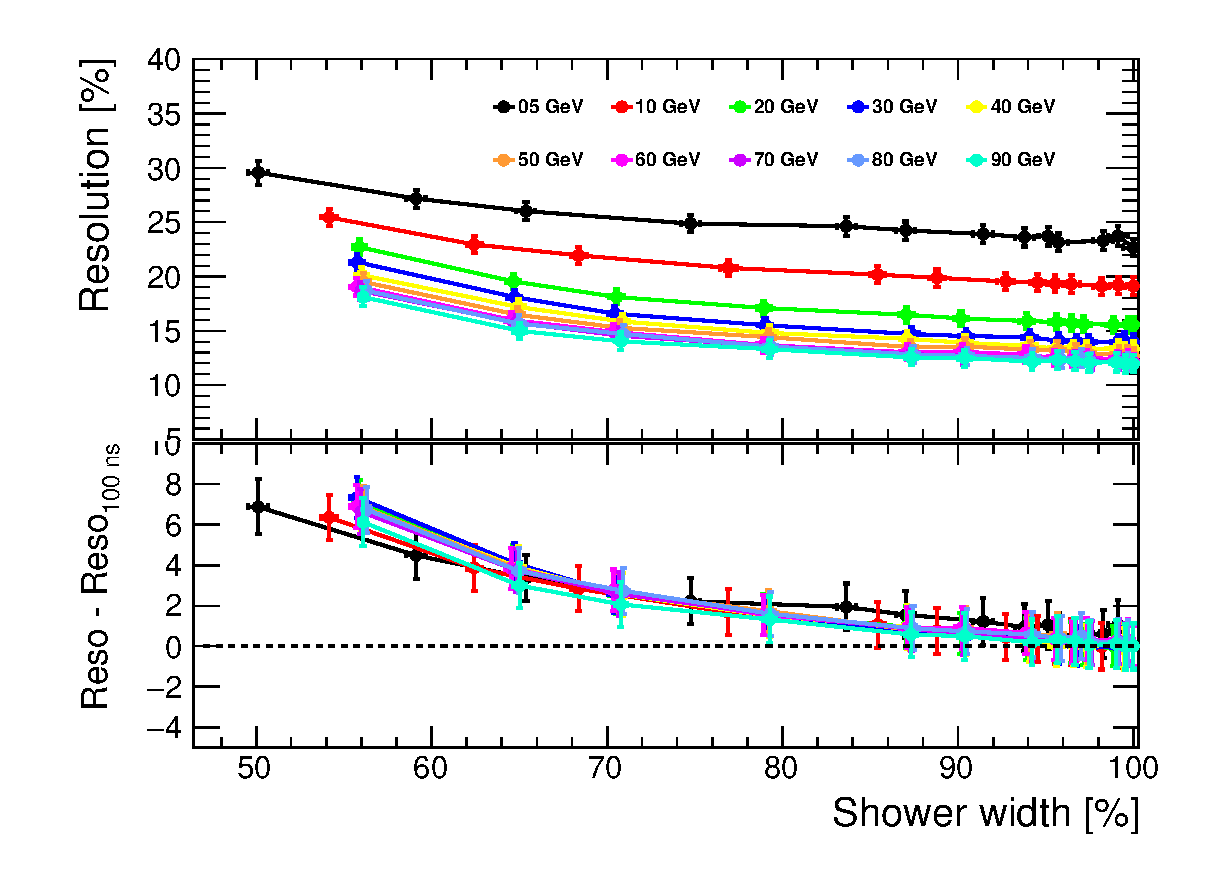
\includegraphics[width=1\linewidth]{../Thesis_Plots/ILD/Smearing_1ns/Plots/ShowerWidth_Resolution_Smearing2.eps}
    \caption{\SI{1}{\nano\second} time resolution.} \label{fig:WidthReso1ns}
  \end{subfigure}
  \begin{subfigure}[t]{0.6\textwidth}
    \centering
    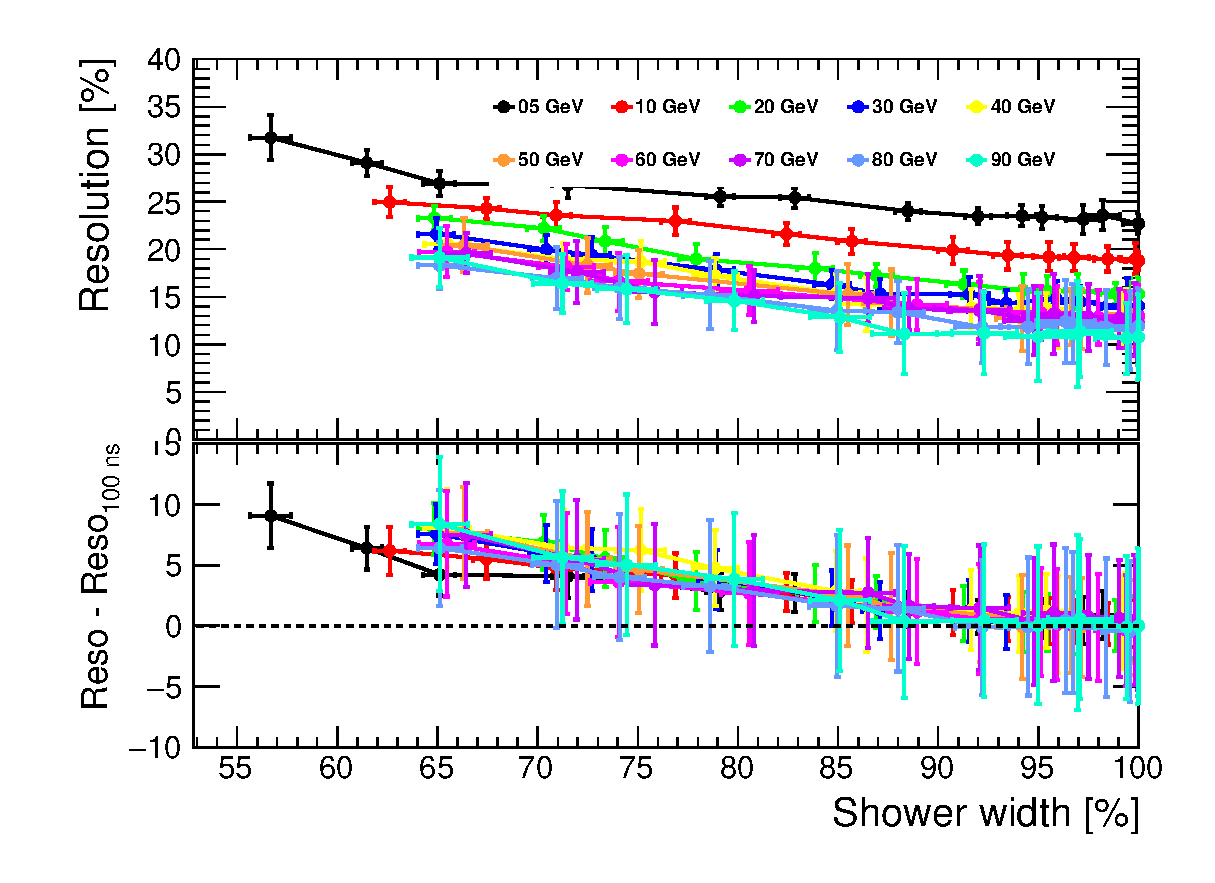
\includegraphics[width=1\linewidth]{../Thesis_Plots/ILD/Smearing_8ns/Plots/ShowerWidth_Resolution_Smearing3.eps}
    \caption{\SI{8}{\nano\second} time resolution.} \label{fig:WidthReso8ns}
  \end{subfigure}
  \caption{Energy resolution as a function of the shower width assuming different time resolutions. The top plot shows the relative energy resolution $\frac{\sigma_{E}}{E}$ for kaons from 5 to 90 \GeV where each point is representing a timing cut as function of the shower width. The bottom plot shows the deviation to the nominal resolution at 100 ns as a function of the shower width. The error bars are statistical uncertainties.}
\end{figure}

From these figures, we can conclude that for a timing resolution of around 1 ns or better, the calorimeter linearity and energy resolution does not get affected much for timing cuts around 5-10 ns. This can be explain because more than 90\% of the energy is deposited within 10 ns. This deposited energy can be identified mostly to the core of the shower in a radius of around 10 cm around the main shower axis. Moreover, the shower width get reduced by around 40-50\%. However, for higher timing resolution, the linearity and energy resolution would get much more affected for timing cuts of 5-10 ns. The shower width can still be reduced by around 30\% for a loss in resolution of around 6-8\% (absolute) and a degradation of the linearity by 20-30\% maximum. One could use timing information in order to improve the pattern recognition efficiently. For example, timing could be used to help in the clustering step in Pandora, especially for nearby close showers. Then a re-clustering step taking into account timing information could be done to recover the loss in energy resolution and linearity. In addition, as the electromagnetic core of the shower is related to quasi-instantaneous energy depositions and the hadronic part of the shower is related to late energy depositions, timing information could be used to improve the energy resolution by software compensation \cite{Benaglia2016}.

\section{Understanding the degradation of the energy resolution with timing cuts}
\label{sec:eresdegrad}

To investigate and understand the degradation of the energy resolution with timing cuts, a simple complementary analysis has been done based on the CAN 028 \cite{CaN028}. The analysis note presents a software compensation method to improve the energy resolution using a correction factor derived from the knowledge of the electromagnetic and hadronic fraction in a shower on an event-by-event basis. It was found that the shape of energy density distributions is correlated with the calorimeter response. The goal of this study is to show that timing cuts favor high electromagnetic fraction events and thus, reduces the correlation.

\subsection{Hit Energy spectra in HCAL}

Due to the high granularity of the HCAL in the ILD detector, a detailed study of hadronic showers is possible at the single cell level (hits). The hadronic calorimeter in ILD is of a non-compensating nature resulting in a higher response for the electromagnetic component of a hadronic shower than for the hadronic component. The $\frac{e}{\pi}$ ratio is around 1.2 \cite{ILC_TDR_Vol4}. Because of this, hadron induced showers with a higher electromagnetic fraction will give a higher response and vice-versa. An example is shown in figure \ref{fig:Response30GeV}. $E_{mean}$ and $\sigma$ correspond to the mean of the distribution and RMS, respectively. The blue subsample contains events reconstructed with $E_{reco} < E_{mean} - \sigma$ and the red one with $E_{reco} > E_{mean} + \sigma$. The corresponding hit energy spectrum is shown in figure \ref{fig:HitSpectra30_100ns}. This shows that the shape of the hit energy spectrum is closely related to the deposited energy. Clusters with a higher reconstructed energy contain hits with larger hit energies which are expected to be mainly caused by the EM component.

\begin{figure}[htbp!]
  \centering
  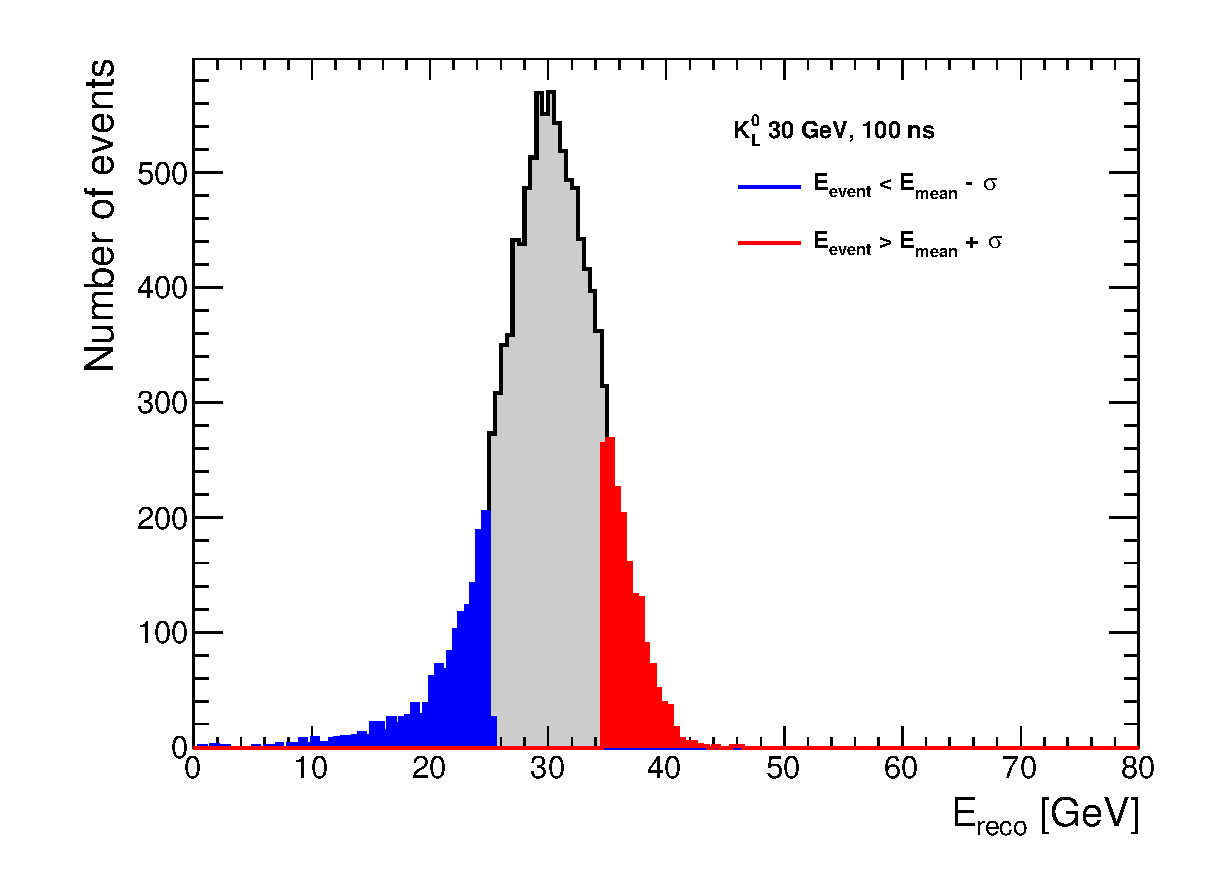
\includegraphics[width=0.6\linewidth]{../Thesis_Plots/ILD/AdditionalPlots/Plots/EnergySum_100ns_30GeV.eps}
  \caption{Reconstructed energy distribution for 30 GeV kaons. The blue sample corresponds to events with $E_{reco} < E_{mean} - \sigma$ and the red sample corresponds to events with $E_{reco} > E_{mean} + \sigma$.} \label{fig:Esum30_100ns}
\end{figure}

Following the CAN 028, a quantitative probability $C_{i}^{lim}$ of the i-th event was obtained as follows:
\begin{equation}
  C_{i}^{lim} = \frac{N_{i}(e \leq e^{lim})}{N_{i}^{HCAL}}
\end{equation}
where $N_{i}(e \leq e^{lim})$ is the number of hits with energy $e \leq e^{lim}$ and $N_{i}^{HCAL}$ the number of hits in the HCAL. The value of $e^{lim}$ is between 3 to 5 MIPs, determined by looking at the intersection of hit energy spectra of the red and blue subsamples for kaons between 10 and 80 GeV. The figure \ref{fig:HitSpectra30_Zoom_100ns} shows the hit energy spectra between 0 and 14 MIP for 30 GeV.

\begin{figure}[htbp!]
  \centering
  \begin{subfigure}[t]{0.49\textwidth}
    \centering
    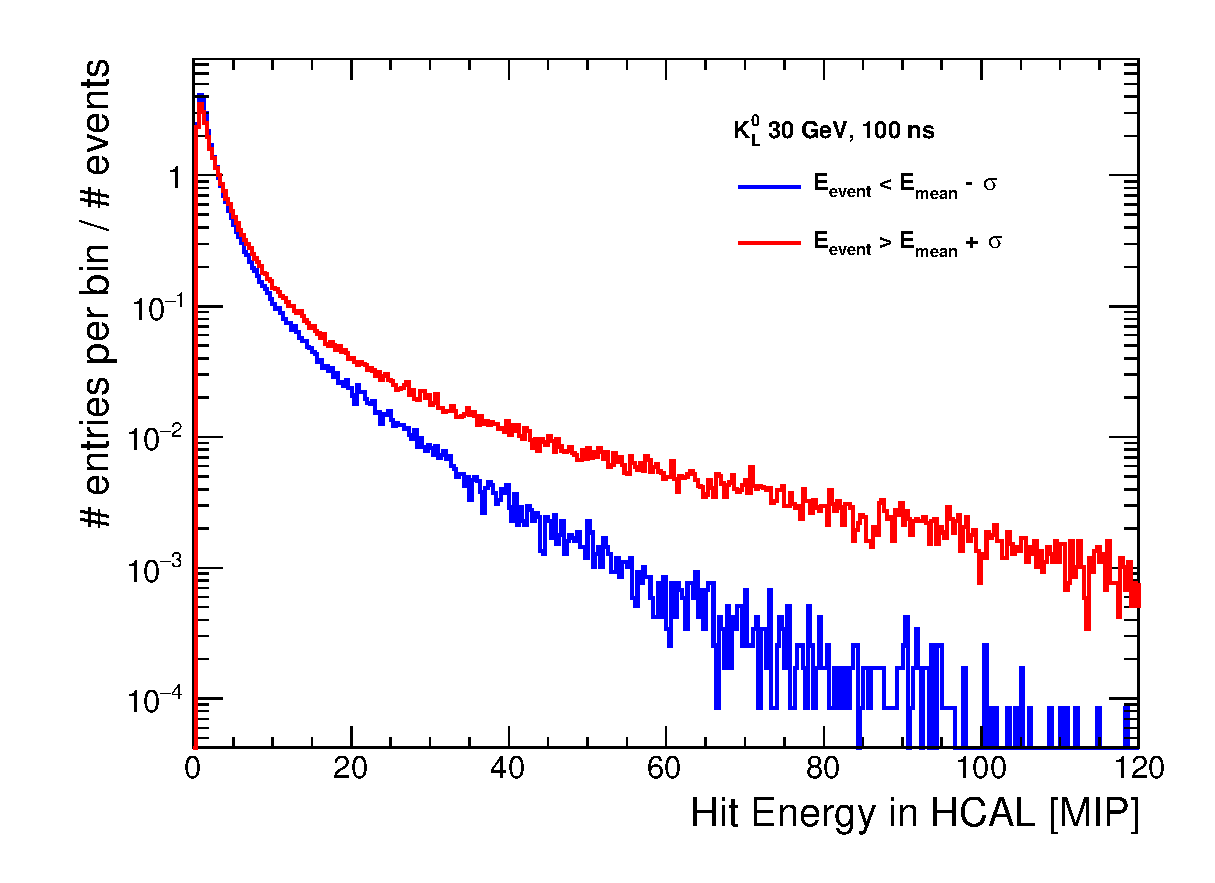
\includegraphics[width=1\linewidth]{../Thesis_Plots/ILD/AdditionalPlots/Plots/HitEnergySpectra_100ns_30GeV.eps}
    \caption{} \label{fig:HitSpectra30_100ns}
  \end{subfigure}
  \hfill
  \begin{subfigure}[t]{0.49\textwidth}
    \centering
    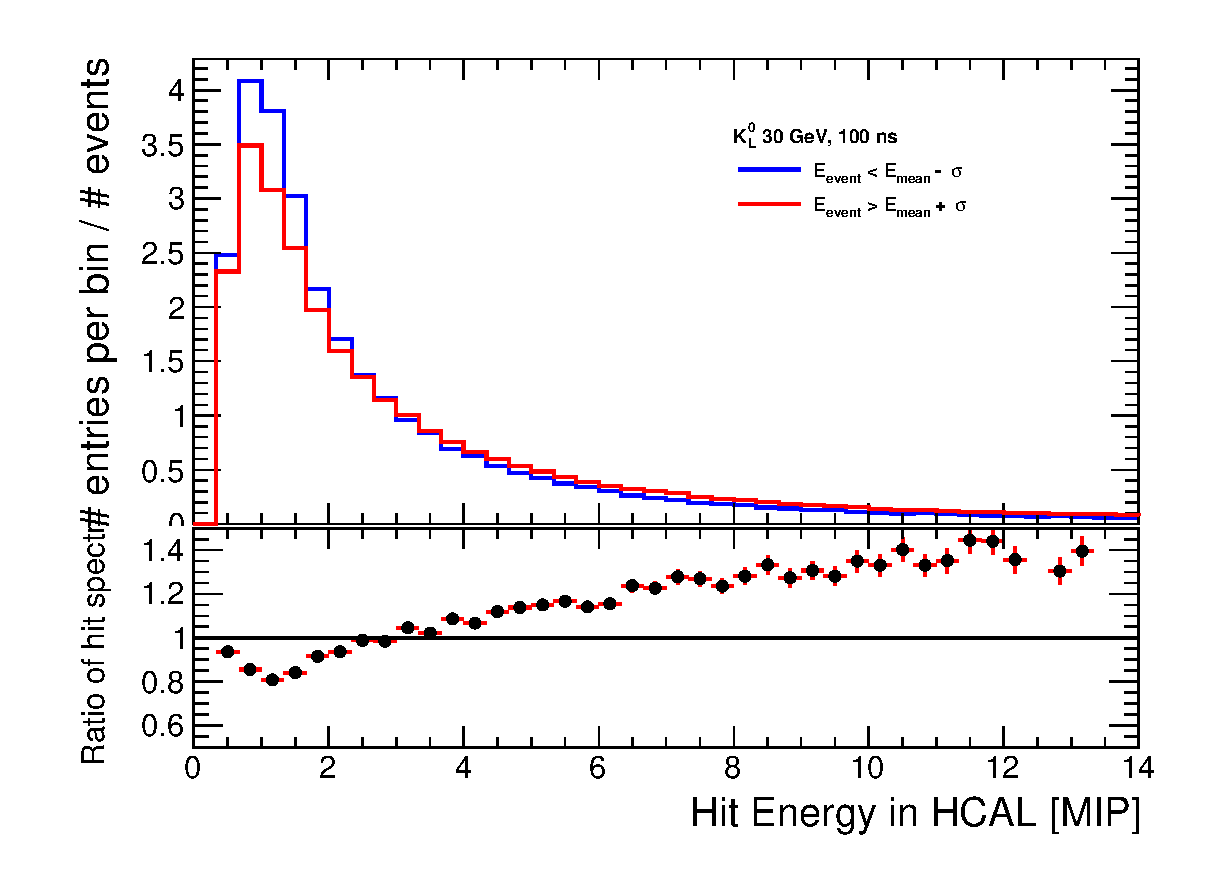
\includegraphics[width=1\linewidth]{../Thesis_Plots/ILD/AdditionalPlots/Plots/HitEnergySpectra_Zoom_100ns_30GeV.eps}
    \caption{} \label{fig:HitSpectra30_Zoom_100ns}
  \end{subfigure}
  \caption{Hit energy spectrum in the HCAL corresponding to subsamples with low (in blue) and high (in red) energy depositions. The left plot is focused in the region between 0 and 14 MIPs. The bottom plot shows the ratio of the red to the blue spectrum that was used to determine the value for $e^{lim}$.} \label{fig:Response30GeV}
\end{figure}

The distribution of $C^{lim}$ for different values of $e^{lim}$ are shown in figure \ref{fig:CLim30_100ns} for 30 GeV kaons. One can see that the distributions get narrower with increasing $e^{lim}$. By choosing the right value of $e^{lim}$, it may be possible to distinguish between the red and blue subsamples by their $C^{lim}$ distributions. For this analysis, a value of 3.5 MIP was chosen for $e^{lim}$. One can observe that events where the reconstructed energy is below $E_{mean} - \sigma$ correspond to a higher value of $C^{lim}$ and vice-versa. The blue distribution has a mean of 0.71 and the red distribution has a mean of 0.61, this corresponds to a separation of 14.1\%. An inverse correlation is found between the total energy in the HCAL and $C^{lim}$ as shown in figure \ref{fig:EhcalCLim30_100ns}. The inverse correlation is much stronger for higher kaon energies and becomes weaker with lower energies.

\begin{figure}[htbp!]
  \centering
  \begin{subfigure}[t]{0.49\textwidth}
    \centering
    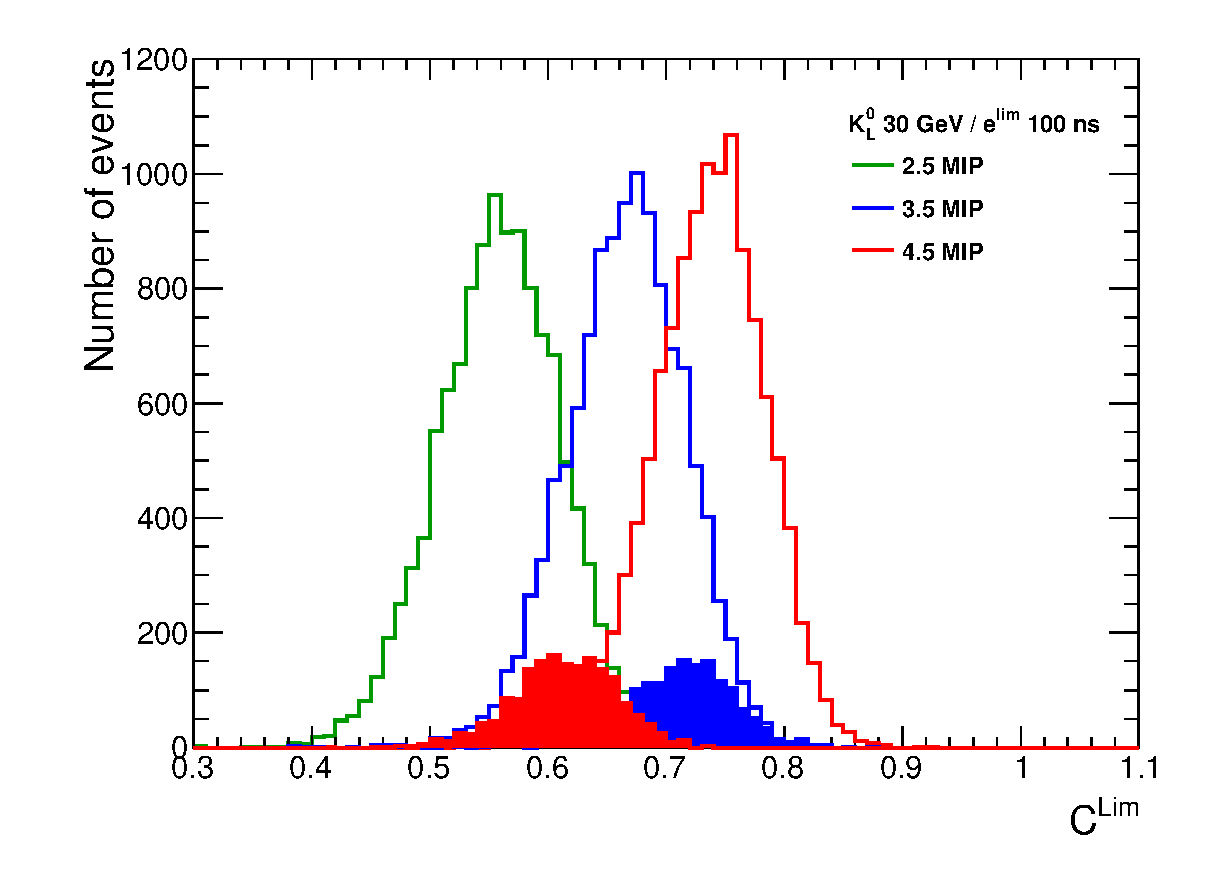
\includegraphics[width=1\linewidth]{../Thesis_Plots/ILD/AdditionalPlots/Plots/CLim_100ns_30GeV.eps}
    \caption{} \label{fig:CLim30_100ns}
  \end{subfigure}
  \hfill
  \begin{subfigure}[t]{0.49\textwidth}
    \centering
    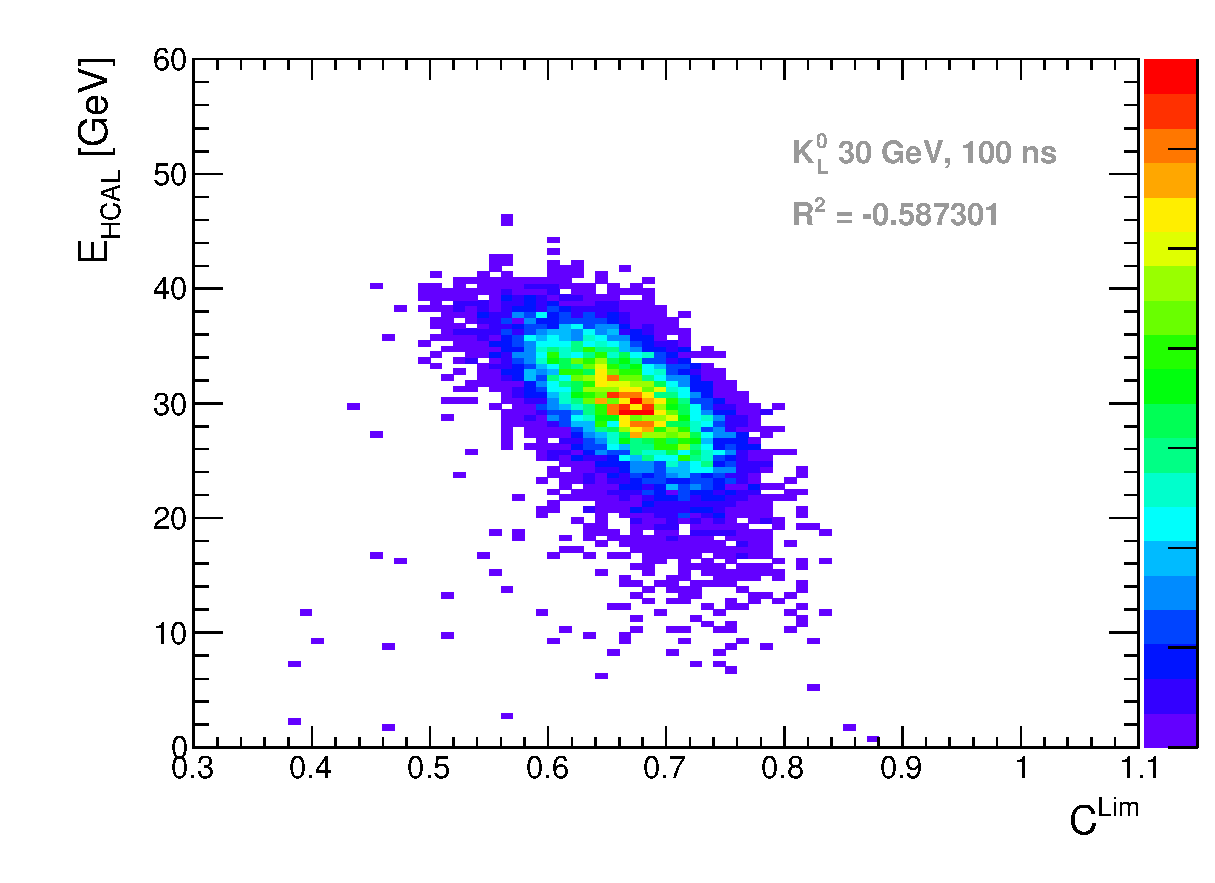
\includegraphics[width=1\linewidth]{../Thesis_Plots/ILD/AdditionalPlots/Plots/EhcalCLim_100ns_30GeV.eps}
    \caption{} \label{fig:EhcalCLim30_100ns}
  \end{subfigure}
  \caption{\subref{fig:CLim30_100ns}) Distributions of $C^{lim}$ for different values of $e^{lim}$ for 30 GeV kaons. The red and blue filled histograms corresponds to events that are in the region $E_{mean} \pm \sigma$ respectively for $e^{lim}$ = 3.5 MIPs. \subref{fig:EhcalCLim30_100ns}) Energy deposited in the HCAL as a function of $C^{lim}$ for $e^{lim}$ = 3.5 MIPs for 30 GeV kaons.}
\end{figure}

In a next step, a timing cut is applied and a comparison with these results is done. It is expected that timing cuts will have an effect of narrowing the $C^{lim}$ distributions, thus bringing the blue $C^{lim}$ distribution (hadronic component) closer to the red $C^{lim}$ distribution (EM component). Therefore reducing the inverse correlation of $C^{lim}$ with the energy deposited. This is due to the fact that fluctuation are cut down by timing cuts, favoring hadronic showers with a higher electromagnetic fraction.

\subsection{Influence of timing cuts on hit energy spectra in HCAL}

A check was performed on the shape of the hit spectra in the HCAL with different timing cuts. The figure \ref{fig:HitSpectra30_timingcuts} shows the hit spectra for 30 GeV kaons with a timing cut of 100 and 1 ns. The green line in the bottom plot represents the value of $e^{lim}$ = 3.5 MIPs.

One can notice that the shape of the spectra differs with timing cuts. A large reduction of low energy hits ($\sim$1 MIP) is visible. With a cut of 1 ns, there are around 10\% less hits over 4 MIPs but up to 60\% less hits below 1 MIP. With a value of 3.5 MIP for $e^{lim}$, it seems that there are globally fewer hits below, thus reducing the value of $C^{lim}$. A lower value of $C^{lim}$ would correspond to a higher energy deposited thus giving a hint that timing cuts enhance the electromagnetic response of the calorimeter making even more non-compensating. This is shown in figure \ref{fig:CLim30_1ns}.

\begin{figure}[htbp!]
  \centering
  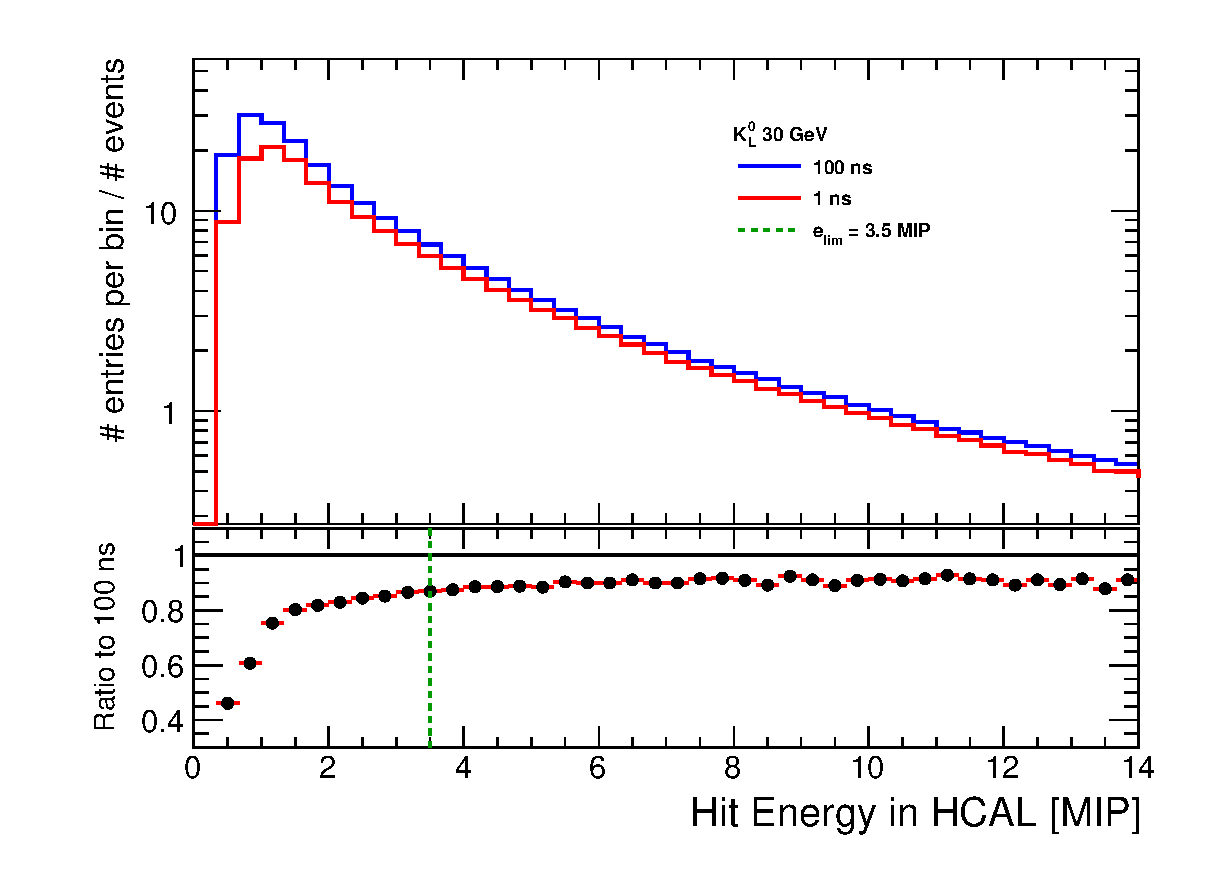
\includegraphics[width=0.6\linewidth]{../Thesis_Plots/ILD/AdditionalPlots/Plots/HitEnergySpectra_Comparison_30GeV.eps}
  \caption{Normalized hit energy spectra in the HCAL for 30 GeV kaons applying a timing cuts of 100 ns in blue and 1 ns in red. The bottom plot shows the ratio of the red spectra to the blue spectra.} \label{fig:HitSpectra30_timingcuts}
\end{figure}

The blue $C^{lim}$ distribution has a mean of 0.66 and the red $C^{lim}$ distribution has a mean of 0.58. This corresponds to a separation of 12.1\%. The timing cut of 1 ns has the effect of reducing the distance between both distributions by around 2\% compared to the nominal 100 ns timing cut. To further confirm this observation, the same correlation plots between the energy deposited in the HCAL and $C^{lim}$ is shown in figure \ref{fig:EhcalCLim30_1ns} for 1 ns timing cut. The anti-correlation is reduced slightly with the correlation coefficient going from -0.58 to -0.48 and the distribution looks more circular. This further confirms that the timing cuts reduce the fluctuations between the electromagnetic and hadronic fractions in hadronic showers by cutting the hadronic response and enhancing the electromagnetic response. This has an effect of non-compensation in the response to hadronic showers, thus degrading the energy resolution furthermore.

\begin{figure}[htbp!]
  \centering
  \begin{subfigure}[t]{0.49\textwidth}
    \centering
    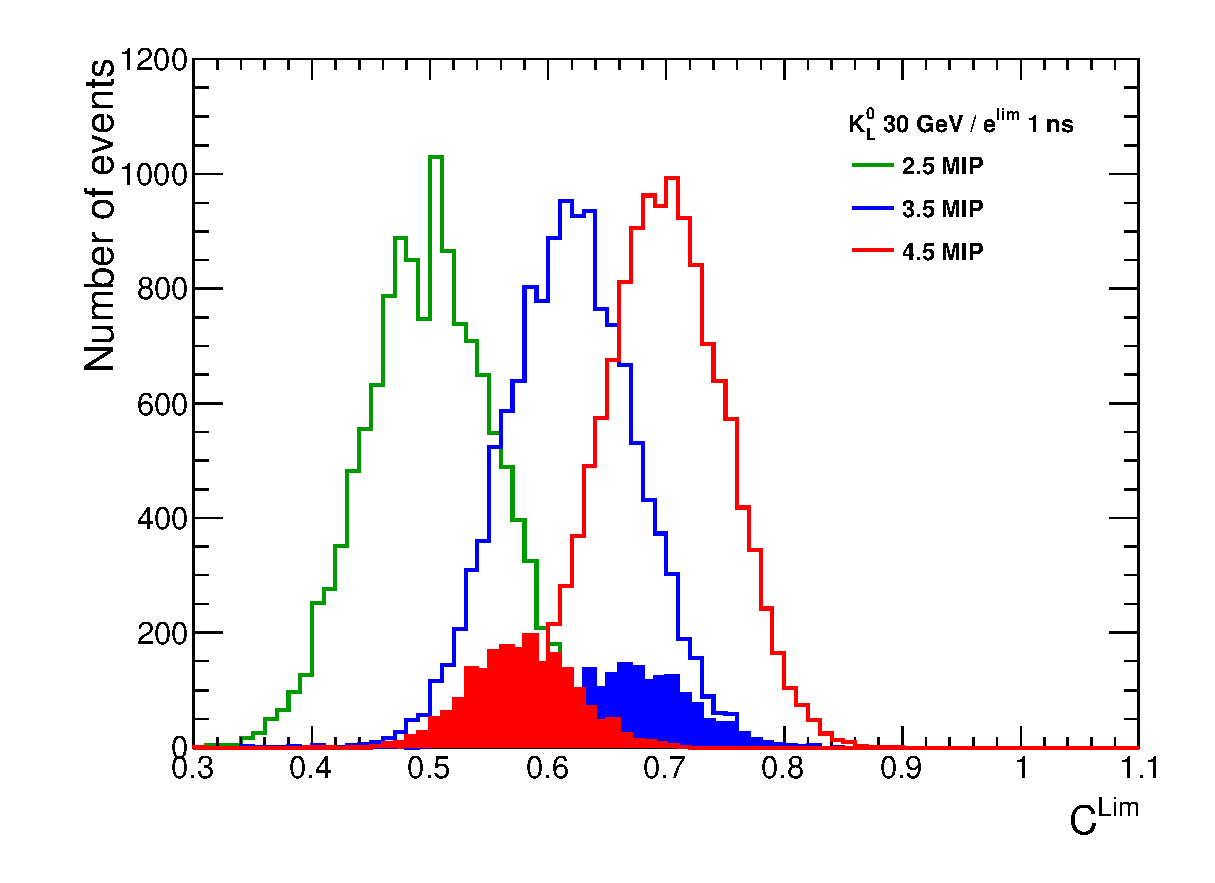
\includegraphics[width=1\linewidth]{../Thesis_Plots/ILD/AdditionalPlots/Plots/CLim_1ns_30GeV.eps}
    \caption{} \label{fig:CLim30_1ns}
  \end{subfigure}
  \hfill
  \begin{subfigure}[t]{0.49\textwidth}
    \centering
    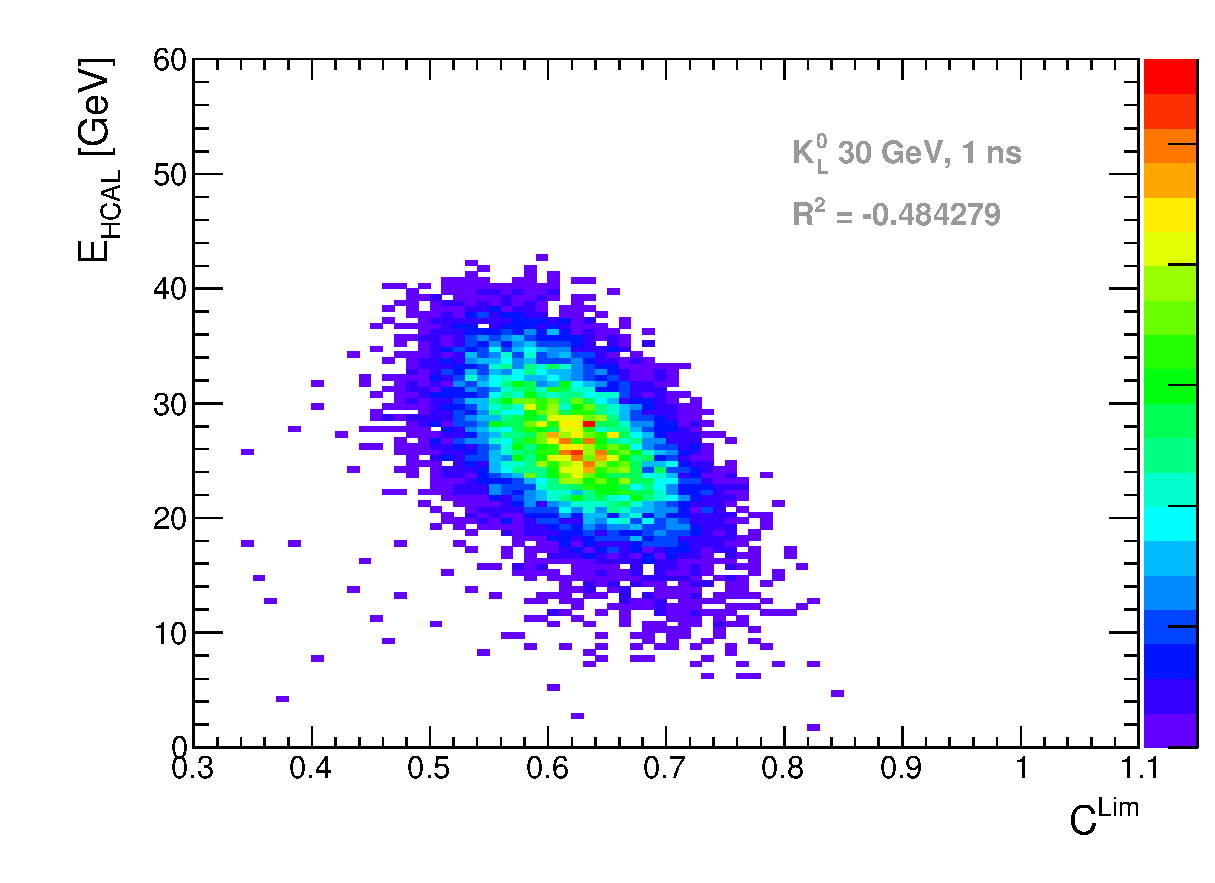
\includegraphics[width=1\linewidth]{../Thesis_Plots/ILD/AdditionalPlots/Plots/EhcalCLim_1ns_30GeV.eps}
    \caption{} \label{fig:EhcalCLim30_1ns}
  \end{subfigure}
  \caption{\subref{fig:CLim30_1ns}) Distributions of $C^{lim}$ for different values of $e^{lim}$ for 30 GeV kaons for a 1 ns timing cut. The red and blue filled histograms corresponds to events that are in the region $E_{mean} \pm \sigma$ respectively. \subref{fig:EhcalCLim30_1ns}) Energy deposited in the HCAL as a function of $C^{lim}$ for $e^{lim}$ = 3.5 MIPs for 30 GeV kaons with a timing cut of 1 ns.}
\end{figure}
